\section{StarDICE response}
\label{sec:rsd}

In this section, we will show the methodology to obtain the \SD telescope response $\Rtel$ from the Equation~\ref{eq:rsd}.

\subsection{Data set description}
\label{sec:sd_datadesc}

As described in section \ref{sec:cbp_datadesc}, the laser emits pulses at a rate of \SI{1}{\kilo\hertz} in bursts that are separated with dark times. Figure~\ref{fig:ccd_examples} shows examples of images obtained when the CBP shoots in the \SD CCD camera with two different pinholes. 

\begin{figure}[h]
    \centering
    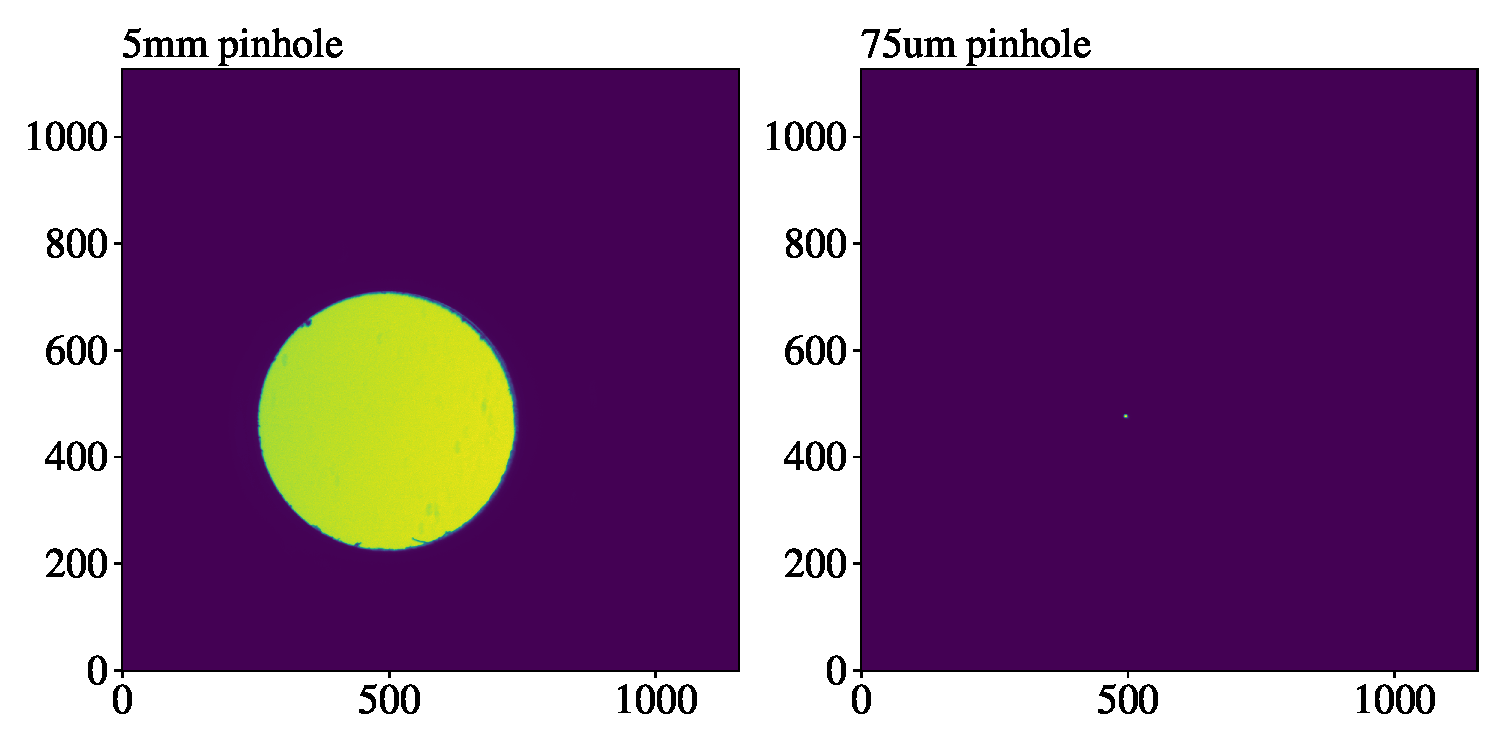
\includegraphics[width=\columnwidth]{fig/ccd_examples.pdf}
    \caption{Examples of images obtained when the CBP shoots in the \SD telescope with the CBP at $\lambda_L=\SI{450}{\nm}$, with the \bpinhole on the right and \spinhole on the left. The ghost reflection is visible for both image at the left of the main spot. In the \bpinhole pinhole image, an annulus around the main spot is visible, and correspond to light diffusion around a mechanical iris at the input of the CBP.}
    \label{fig:ccd_examples}
    %~/stardice/analysis/cbp_paper/total_fluxes/ghost_stack_figure.ipynb
\end{figure}

\subsection{Reduction of images}
\label{sec:photometry}

Firstly, we need to subtract the overscan in every image. The mean of each column $i$ of the horizontal overscan and each row $j$ of the vertical overscan is computed. For each pixel $(i, j)$, we subtract the sum of estimation of the overscan estimated on the column $i$ and the row $j$.
Then, aperture photometry is done to extract the cumulated charge from the \SD camera images. This requires a background subtraction, and two differents methods are used depending on the pinhole.

\subsubsection{\spinhole pinhole}

To estimate the background contribution, the sources in the image need to be detected and masked. We compute the standard deviation of an image $\sigma$, and every pixel with a signal higher than 5$\sigma$ is masked, as well as all the surrounding pixels that has a signal higher than 2$\sigma$. Then we proceed to a segmentation of the masked image into boxes of $129\times132$ pixels. We compute the mean and the standard deviation of the background in each of these boxes, and we interpolate their values in a 2D map to get our estimation of the background. This background estimation is subtracted to the image. Then, the centroid of the spot of interest is computed to pursue aperture photometry at this position. The number of charges $\Qccd$ is measured with aperture photometry at a radius of 20.8 pixels for every image of the dataset with the \spinhole.

\subsubsection{\bpinhole pinhole}

When using \bpinhole pinhole, the main spot take a significant area of the focal plane, meaning there is not enough background in the image to reconstruct it. The background is estimated with dark exposures with the laser off. These dark images are stationary with respect to time and wavelength, and the spatial mean of all these dark images dark is computed to obtain a master dark. The background contribution is estimated by aperture photometry in the master dark at the same position and same radius than the classic images. We find the centroid of the spot of interest, and we measure the charges $\Qccd^{\bpinhole}$ collected in the \SD camera by aperture photometry, subtracted of the background contribution. The optimal radius is evaluated at 300 pixels for the \bpinhole pinhole in order to contain the main spot and the 1\up{st} order ghost. It could be discussed to contain the iris diffusion, but the iris flux contribution would be about the same order of magnitude than the shotnoise, so it is decided to not do this.

\subsection{Modelisation of the \SD data for \spinhole pinhole}

%I. model
%difficulté : PSF : convolution ouverture bizarre + réflexions
%on peut modéliser à grande distance : addition moffat + réflexions dans l'optique + ghost 
%description du ghost (2 dans l'infrarouge)
%modélisation courbe de croissance --> plot résultats
%bkg --> cohérent avec darks
%5eme panneau --> chi2/dof

\subsubsection{Description of the model}

In this section, we develop a modelisation of the \spinhole pinhole data, considering that the \SD telescope PSF can be modelized as a Moffat distribution \citep{moffat}. Thus, the core of the spot in the CCD is the convolution of the PSF, the CBP output shape and ghosts from light reflections between the glass before the CCD and the CCD itself, as schematized in Figure~\ref{fig:schema_ghost}. These contributions are making the core of the spot really complex to modelize. However the tail of the PSF should not be impacted by the contribution of the CBP output shape and the light diffusion, so it is expected to behave like a Moffat distribution. The flux $F(r, \lambda)$ measured in the CDD with aperture photometry at a radius $r$ and a wavelength $\lambda$, can be modelized as: 

\begin{equation}
F(r, \lambda) = \frac{A(\lambda) \times M(r, \lambda) + \Kghostfit(r, \lambda)}{1 + \Kghostfit(r \rightarrow +\infty, \lambda)} + \bkg(r, \lambda),
\label{eq:moffat_model}
\end{equation}
with $A(\lambda)$ the total amplitude, $\Kghostfit(r, \lambda)$ the relative contribution of the 1\up{st} order ghost to $A(\lambda)$, $\bkg(r, \lambda)$ the contribution of the background and $M(r, \lambda)$ the moffat distribution defined as:

\begin{equation}
M(r, \lambda)= \left( 1+\frac{r^2}{\alpha(\lambda)^2} \right)^{-\beta(\lambda)},
\end{equation}
with $\alpha(\lambda)$ and $\beta(\lambda)$ the parameters of the Moffat distribution.
The core of the model is fitted on aperture photometry for a radius $r=\SI{20.9}{pixels}$, and then annulus of external radius from \SI{24.9}{pixels} to \SI{419.1}{pixels}. These radius are regularly spaced on a logarithm scale shown in Figure~\ref{fig:ghost_contrast}. The parameters of the fit are adjusted with the \spinhole pinhole dataset No.~8 from Table~\ref{tab:schedule}. To take in account $\Kghostfit(r, \lambda)$, an additive value is set free for every annulus that contains a ghost contribution. The evolution of the Moffat distribution is expected to be smooth with respect to wavelength. So the parameters $\alpha(\lambda)$ and $\beta(\lambda)$ are developed on a B-spline basis with 20 wavelength nodes regularly spaced between \SI{350}{\nano\meter} to \SI{1100}{\nano\meter}. The same goes for the parameters $\Kghostfit(r, \lambda)$ as it corresponds to light reflections on surfaces in the optical path. The results of this fit is shown Figure~\ref{fig:result_params}. 

The $\alpha(\lambda)$ and $\beta(\lambda)$ parameters of the PSF are stable within \SI{350}{\nano\meter} and \SI{950}{\nano\meter}, and change significantly beyond. This is correlated with a change of the PSF shape in the infrared as it can be seen in the image stacks in Figure~\ref{fig:ghost_contrast}. The third panel shows a constant background against wavelength, with a mean of \SI{0.267}{ADU/pixel}. This panel shows also the result of a study over dark images, detailed in Section~\ref{sec:bkg}. The fourth panel presents the ratio $\Kghostfitfirst(\lambda) = \frac{G_1(\lambda)}{A(\lambda)}$ in percent, superimposed with the fraction $\Kghost=\frac{G_1}{G_0}$ obtained by photometry measured on $G_1$. This study is detailed in Section~\ref{sec:ghost}. The reduced chi-squared of the fit in the fifth panel shows that the model is a satisfactory description of the dataset.

\begin{figure}[h]
    \centering
    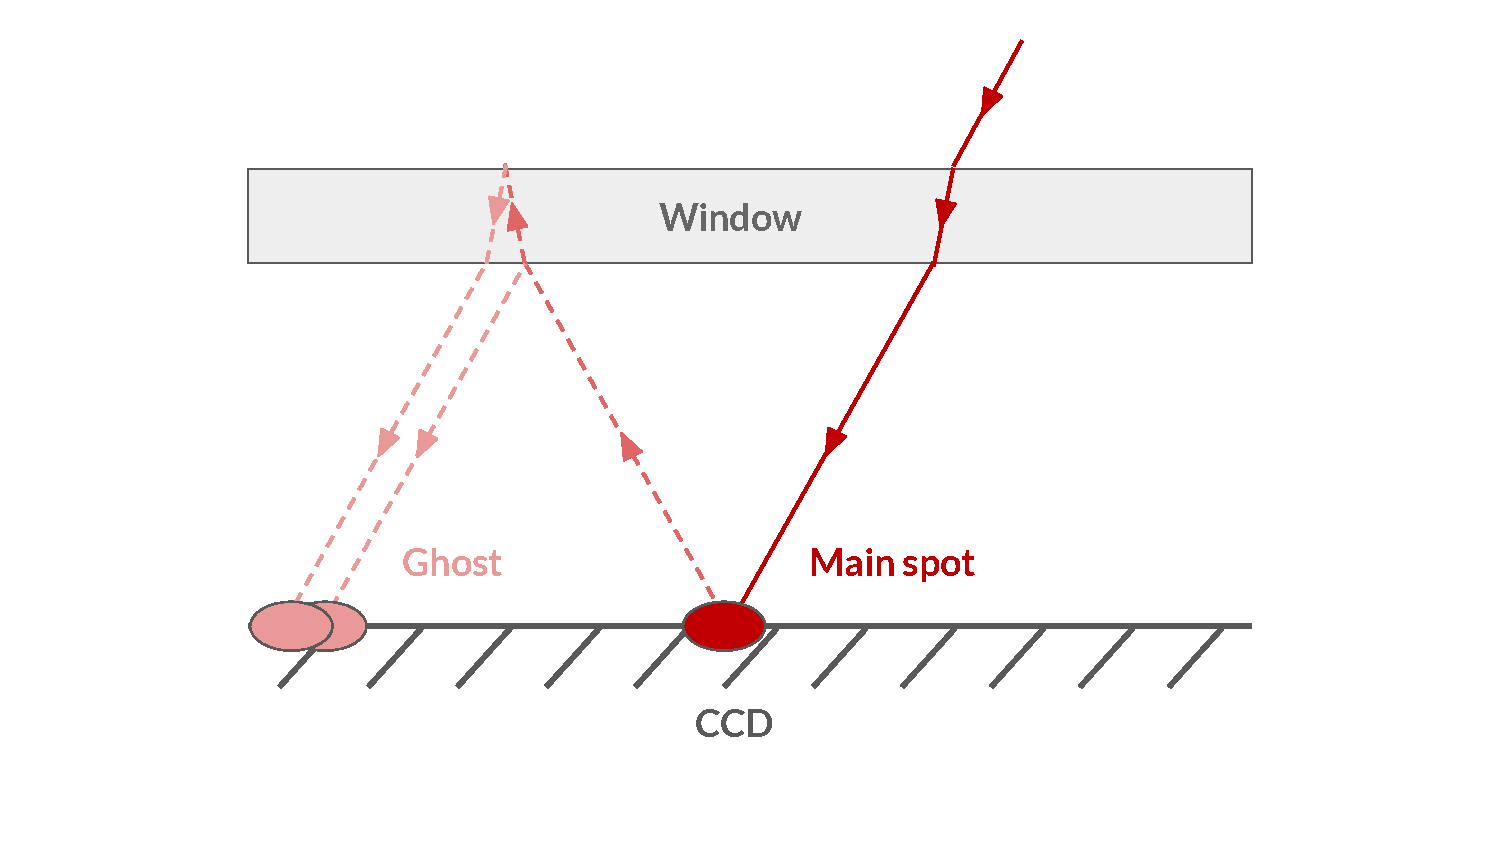
\includegraphics[width=\columnwidth]{fig/schema_ghost.pdf}
    \caption{Schematic of the light reflections that generates the ghosts, which are defocused and less intense images at other positions in the focal plane. The window and the CCD reflections $R_\mathrm{win}$ and $R_\mathrm{ccd}$ being non-zeros, a fraction of the light is reflected at the different interfaces and can be absorbed. $G_0$, $G_1$ and $G_2$ are repsectively the main spot, the 1\up{st} order ghost and the 2\up{nd} order ghost.}
    \label{fig:schema_ghost}
    %Google slides
\end{figure}

\begin{figure}[h]
    \centering
    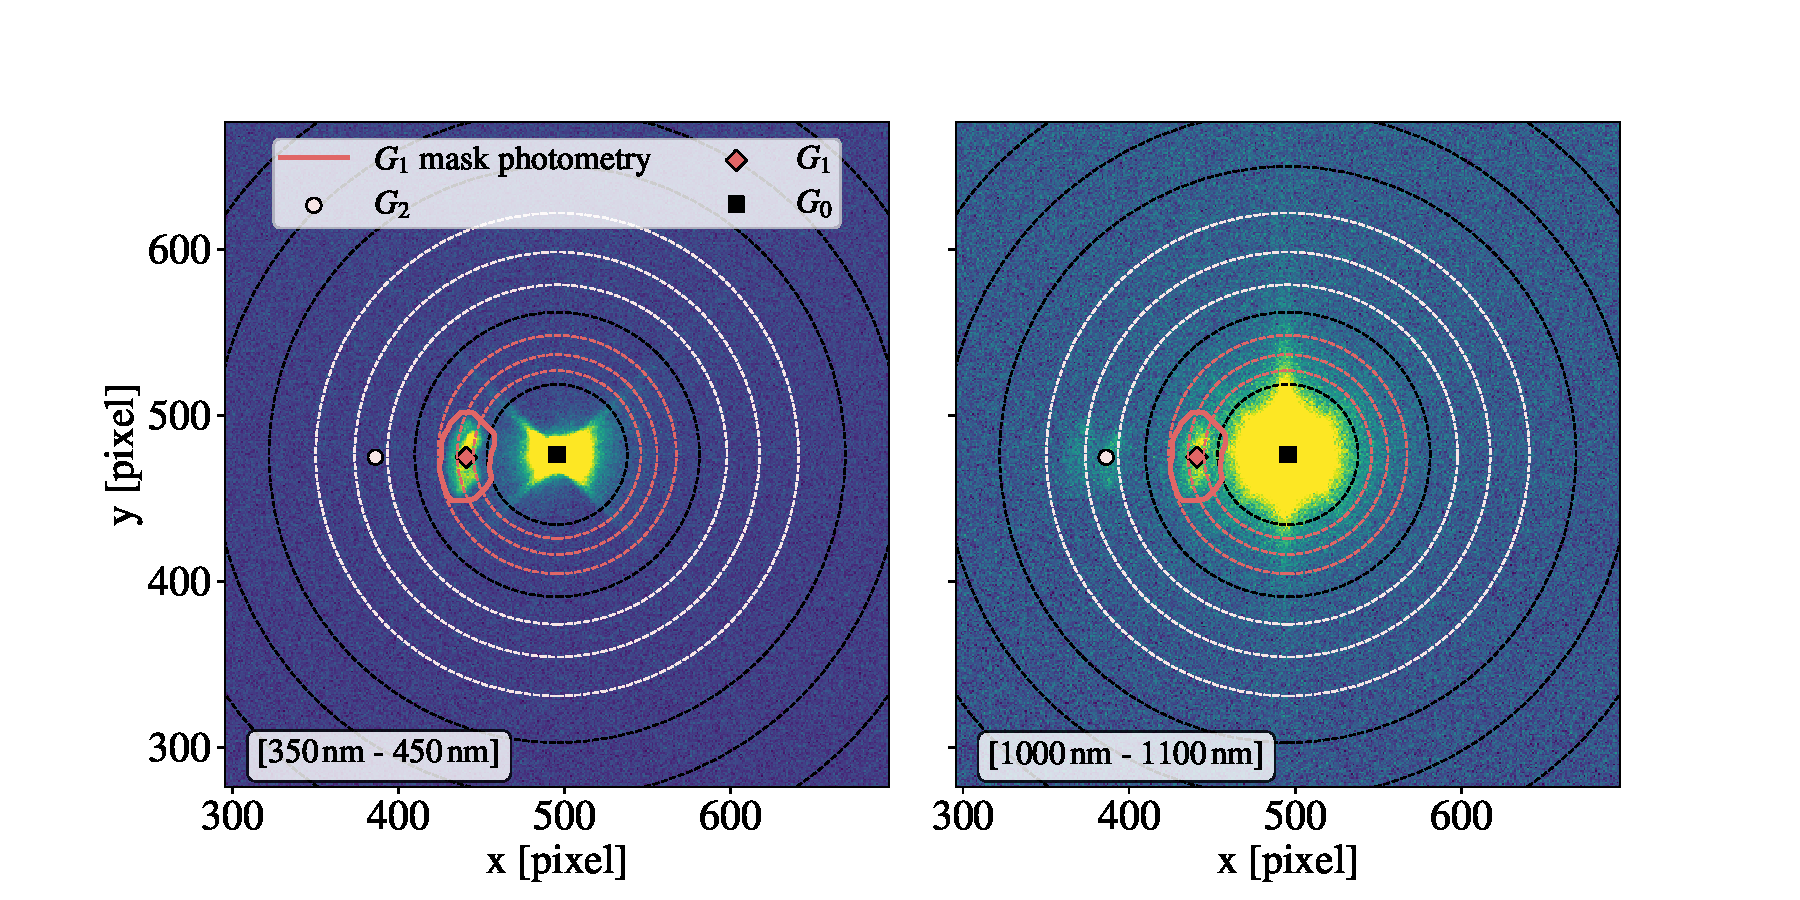
\includegraphics[width=\columnwidth]{fig/ghost_contrast.pdf}
    \caption{Left: Stack of images between \SI{350}{\nano\meter} and \SI{450}{\nano\meter}. The main spot $G_0$ is at the center, and the ghosts reflections at its left. The scale is set on the ZScale from IRAF to make the ghosts visible. The circle corresponds to the aperture photometry at different radius, colored with respect to the order of the ghost when the annulus contains ghost contribution. The red area around the 1$\up{st}$ order ghost represent the area where the photometry of the ghost is measured. Right: Same image but for a stack of images between \SI{1000}{\nano\meter} and \SI{1100}{\nano\meter}. We note that the 2$\up{nd}$ order ghost is not visible for the stack in the UV, where the 1$\up{st}$ order is maximal, while it is visible in the IR, where the 1$\up{st}$ order is lower. For the stack in IR, we osberve the degradation of the \SD PSF.}
    \label{fig:ghost_contrast}
    %~/stardice/analysis/cbp_paper/total_fluxes/ghost_stack_figure.ipynb
\end{figure}

\begin{figure}[h]
     \centering
     \resizebox{\hsize}{!}{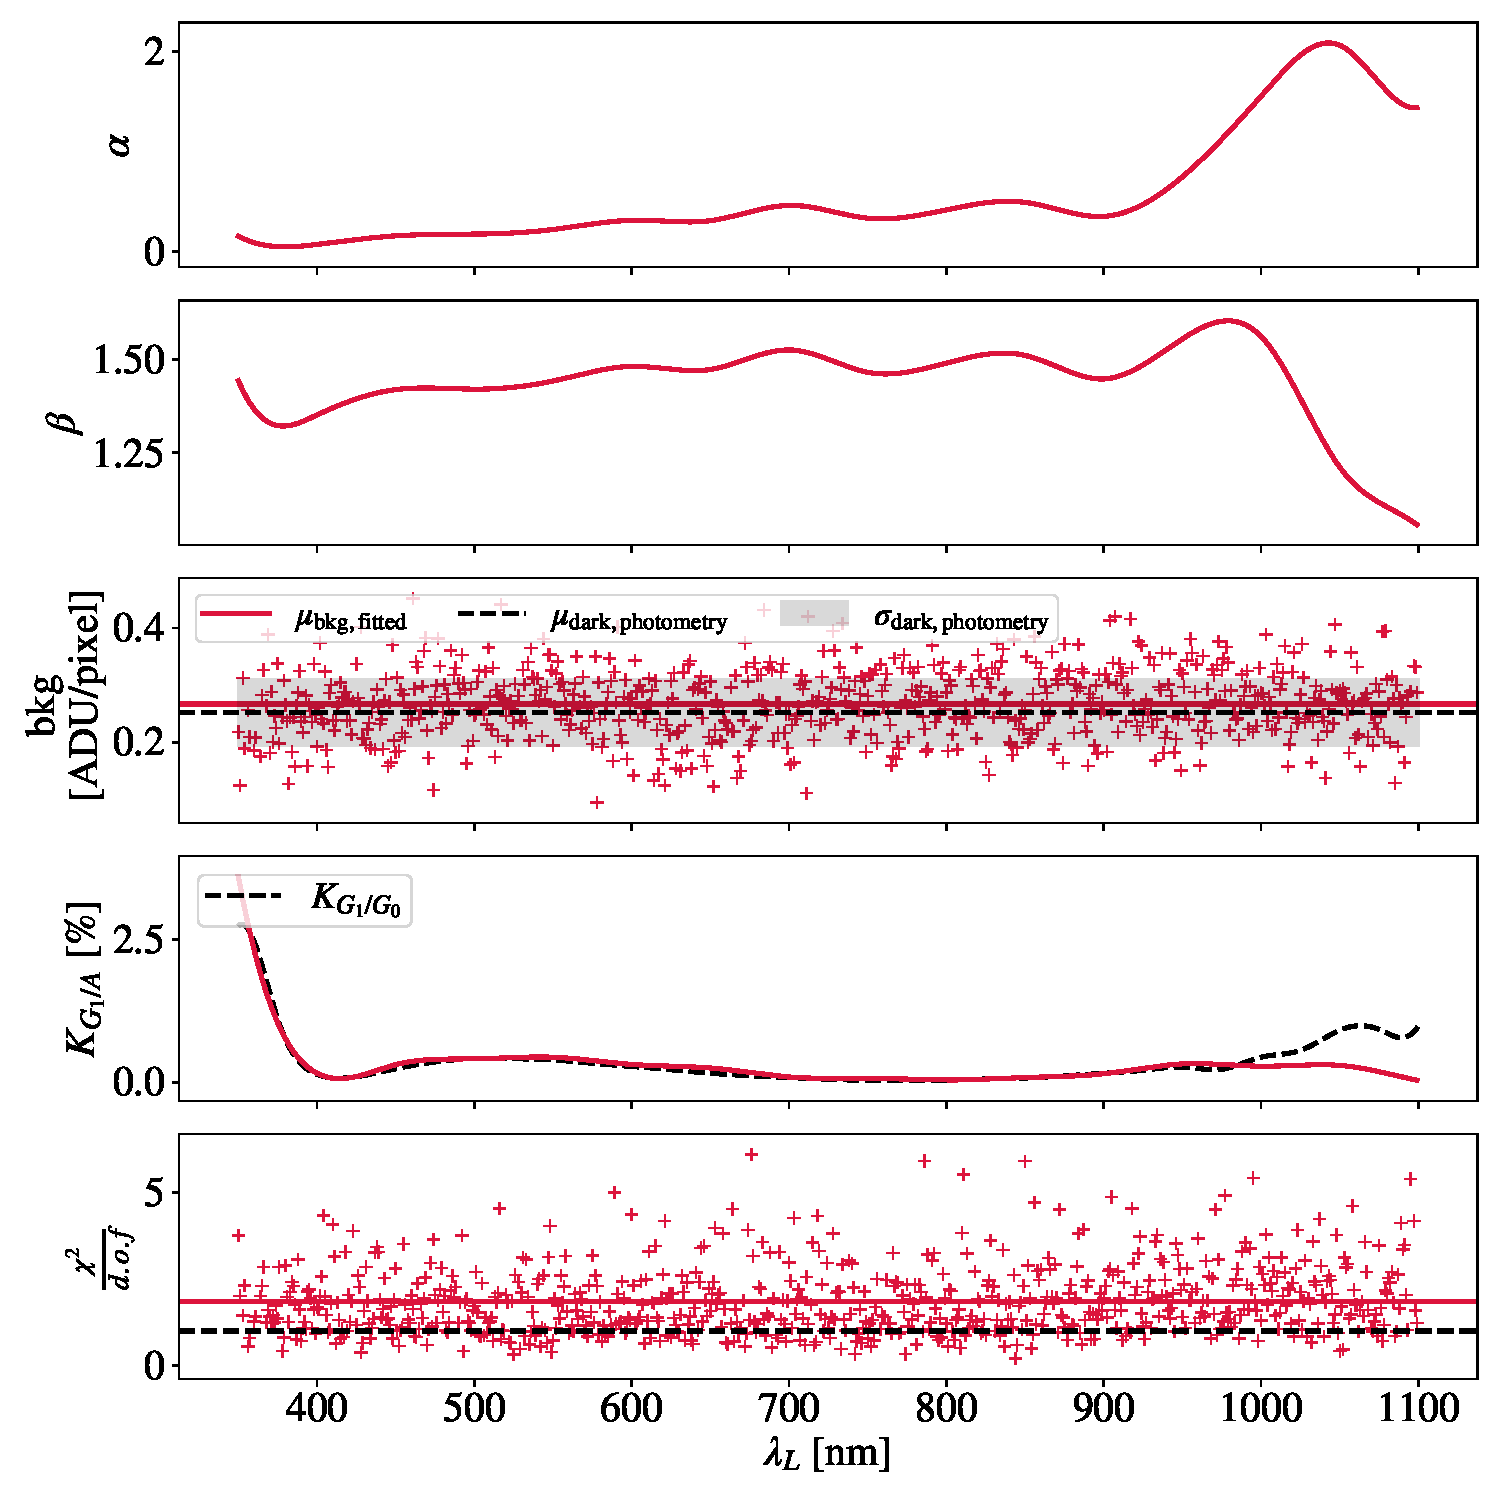
\includegraphics{fig/result_params.pdf}}
     \caption{Result of fit of the model of Equation~\ref{eq:moffat_model}. From top to bottom: the first and second panel represent respectively the $\alpha(\lambda)$ and $\beta(\lambda)$ parameters from the Moffat distribution; the third panel represent the background contribution per pixel; the fourth panel represents $\Kghostfit(\lambda)$, and $\Kghost$; the fifth panel represents the reduced chi-squared of the fit.}
     \label{fig:result_params}
    %~/stardice/analysis/cbp_paper/total_fluxes/fit_results.ipynb
\end{figure}

\subsubsection{Background estimation}
\label{sec:bkg}

As shown in the third panel of Figure~\ref{fig:result_params}, the mean background fitted $\mu_\mathrm{bkg}=0.267$, with a standard deviation of $\sigma_\mathrm{bkg}=0.059$. On the other hand, two datasets of dark images have been studied. Firsly the dark images when shooting with the \bpinhole pinhole from the dataset No.~8 in Table~\ref{tab:schedule}, and secondly dark images when masking the CBP output with a cap from dataset No.~9 in Table~\ref{tab:schedule}. Both datasets are uniform with respect to time and wavelength, and their mean value of ADU/pixel are compatible. We combine this into one dataset of darks and compute their mean $\mu_\mathrm{dark}$ and standard deviation $\sigma_\mathrm{dark}$ in the third panel of Figure~\ref{fig:result_params}. We conclude that the estimation of the background with the fit is consistent with the background datasets results.

\subsubsection{$G_1$ photometry}
\label{sec:ghost}

Let be $G_0(\lambda)$ the quantity of light collected in the main spot, and $G_\mathrm{n}(\lambda)$ the quantity of light collected in the ghost of order $n$. We define $\Kghost$ the ratio of the 1\up{st} order ghost $G_1(\lambda)$ over the main spot $G_0(\lambda)$:

\begin{equation}
    \Kghost = \frac{G_1(\lambda)}{G_0(\lambda)}
    \label{eq:ratio_ghost}
\end{equation}

We measure $G_1(\lambda)$ with the \spinhole pinhole where it is well separated from $G_0(\lambda)$. We build a mask with the expected ghost shape like shown in Figure~\ref{fig:ghost_contrast}, and we fit its best position on the image. To estimate the background at this position, we assume that the main spot has a spatial vertical symmetry, and measure the ADUs contained in a symmetric mask at the vertical symmetric position from the main spot. Then, $G_1(\lambda)$ is the sum of the ADUs in the ghost mask after background subtraction. On the other hand, $G_0(\lambda)$ is measured with the aperture photometry described in \ref{sec:photometry}. This study is pursued for the 3 runs of dataset No.~4, and 2 runs of dataset No.~2 from Table~\ref{tab:schedule}. The results obtained for $\Kghost$ are shown in Figure~\ref{fig:ghost_ratio}. 

The ratio $\Kghost$ and $\Kghostfitfirst$ obtained with two different methods are superimposing well below \SI{950}{\nano\meter} in the third panel of Figure~\ref{fig:result_params}, which gives us confidence about tue accuracy of this measurement. Above \SI{950}{\nano\meter} the PSF is deteriorating and starts to overflow in the ghost mask, plus there are interference fringes appearing in the focal plane. These issues can explain the deviation between the two measurements at these wavelengths. The fit result gives more confidence in its accuracy because it deals with the PSF evolution.

\begin{figure}[h]
     \centering
     \resizebox{\hsize}{!}{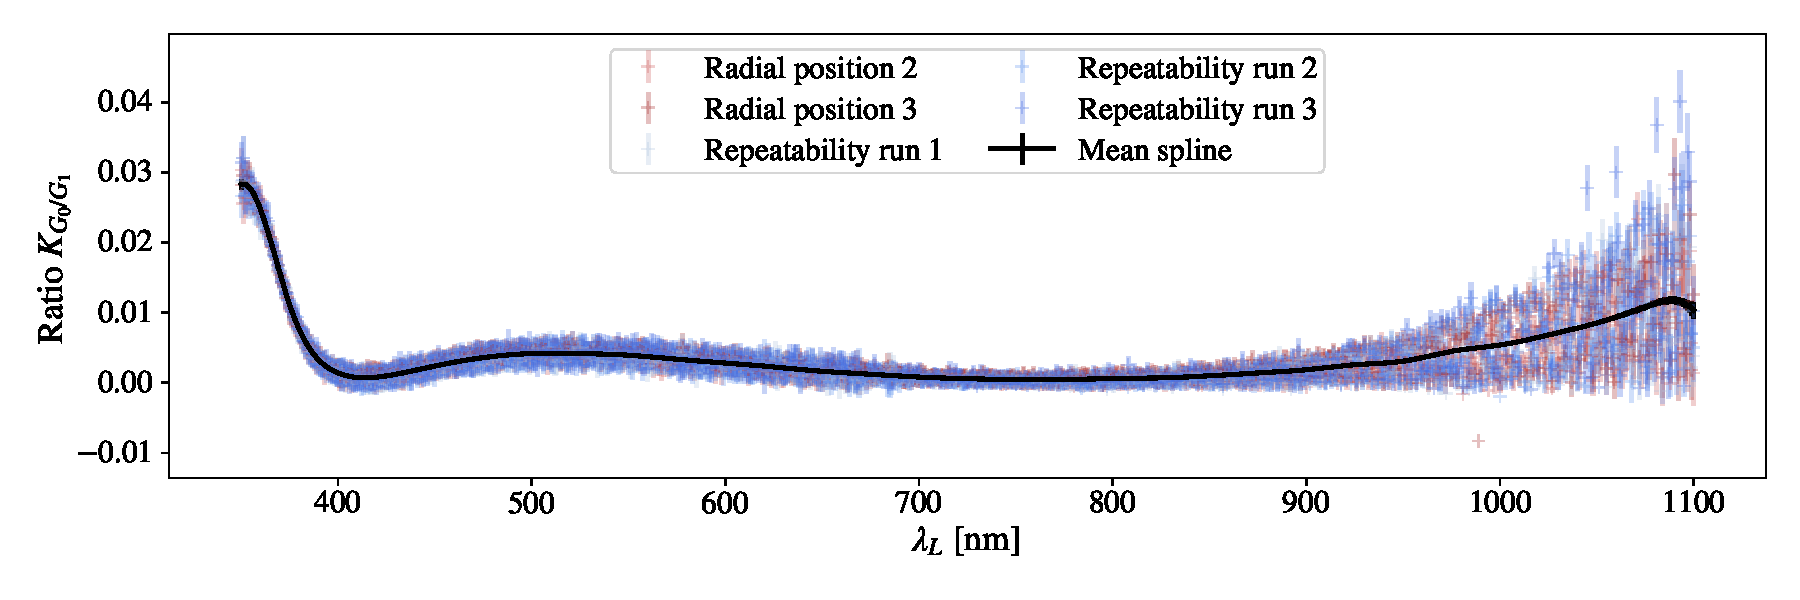
\includegraphics{fig/ghost_ratio.pdf}}
     \caption{Ratio $\Kghost$ with respect to $\lambda_L$. The mean spline goes through the five datasets.}
     \label{fig:ghost_ratio}
    %~/stardice/analysis/cbp_paper/golden_sample_analysis/dr2/ghost_photometry_general.ipynb
\end{figure}

Further investigation indicates that the ghosts of higher order $G_{n>1}$ should contribute for less than $0.1\%$ of $G_0(\lambda)$. Yet, a second order ghost is visible for the stack in infrared in the right panel of Figure~\ref{fig:ghost_contrast}. The reflectivities of the window and the CCD cannot explain this phenomenon, so it has necessarily went through another optical path. The infrared light could have gone through the CCD and reflect in the back of it before being collected.

\subsection{Choice for baseline photometry}

%II. photométrie portable sur ciel 
%
%on peut modéliser pcq on n'a pas de fond --> propre aux images CBP (pas de fond ciel, source isolée), donc peut pas faire en pratique sur ciel
%
%comme d'hab : soustraction de fond classique et se limiter à ouverture donnée ~20 pixels
%si on fait ça, voilà la fraction du flux qu'on récupère : plot de correction d'ouverture phi20/A (quantifier les biais sur F(20)/A et ap_bkg ou fit_bkg), biais à cause du flux perdu et biais à cause de la source  
%
%Problèmes IR:
%1) params fitté partent aux fraises dans l'IR, ça doit venir de StarDICE, peut-être transparence du télescope (regarder dans le filtre y comparé au filtre g ou i) --> peut pas reconstruire de manière précise le flux d'une étoile au-delà de 1000nm (pas de lien entre CBP et obs stardice)
%
%On va mesurer l'ensemble des spots CBP avec l'ouverture à 20 pixels sachant que dans l'IR c'est pas fou 
%*98\% du flux stable en couleur

The modelisation of the image at long distance from the target is possible because of the ideal conditions of these images. These conditions are intrisinc to CBP images, with an isolated source and no sky background, and the possibility to turn off the light. It is impossible to port this method with on-sky data. We choose to carry out the whole analysis with aperture photometry and the background estimation described in Section~\ref{sec:photometry} for the \spinhole pinhole, as it is reproducible with on-sky data. The fraction of flux missed by this method compared to the total amplitude $A$ is quantified in Figure~\ref{fig:bias_aperture}. 

Approximately 2\% of the flux is missed between \SI{400}{\nano\meter} and \SI{900}{\nano\meter}. Below \SI{400}{\nano\meter} the ghost contribution is missed when using an aperture of \SI{20.9}{pixels} and the fraction of flux missed reach 3\%. Above \SI{900}{\nano\meter} where the PSF is degrading, the fraction of flux missed increase by two order of magnitude and reach more than 75\%. The bottom panel of Figure~\ref{fig:bias_aperture} show that aperture photometry is compatible to the fit estimation at less than 0.1\% when the background is estimated with dark datasets. The baseline background estimation induce a bias of approximately 0.1\% between \SI{400}{\nano\meter} and \SI{900}{\nano\meter}.

We can reach the conclusion that the baseline aperture photometry for the \spinhole pinhole can be used for the range between \SI{400}{\nano\meter} and \SI{900}{\nano\meter}. Below \SI{400}{\nano\meter} there is a need to take care of the ghost contribution. Above \SI{900}{\nano\meter}, this method does not measure a representative flux of the target. It is believed that the \SD telescope is the one responsible for the PSF degradation, one possible explanation is that the primary mirror is becoming partially transparent and generate defocused light. Anyhow, the CBP measurements cannot be trusted in this wavelength range. 

\begin{figure}[h]
     \centering
     \resizebox{\hsize}{!}{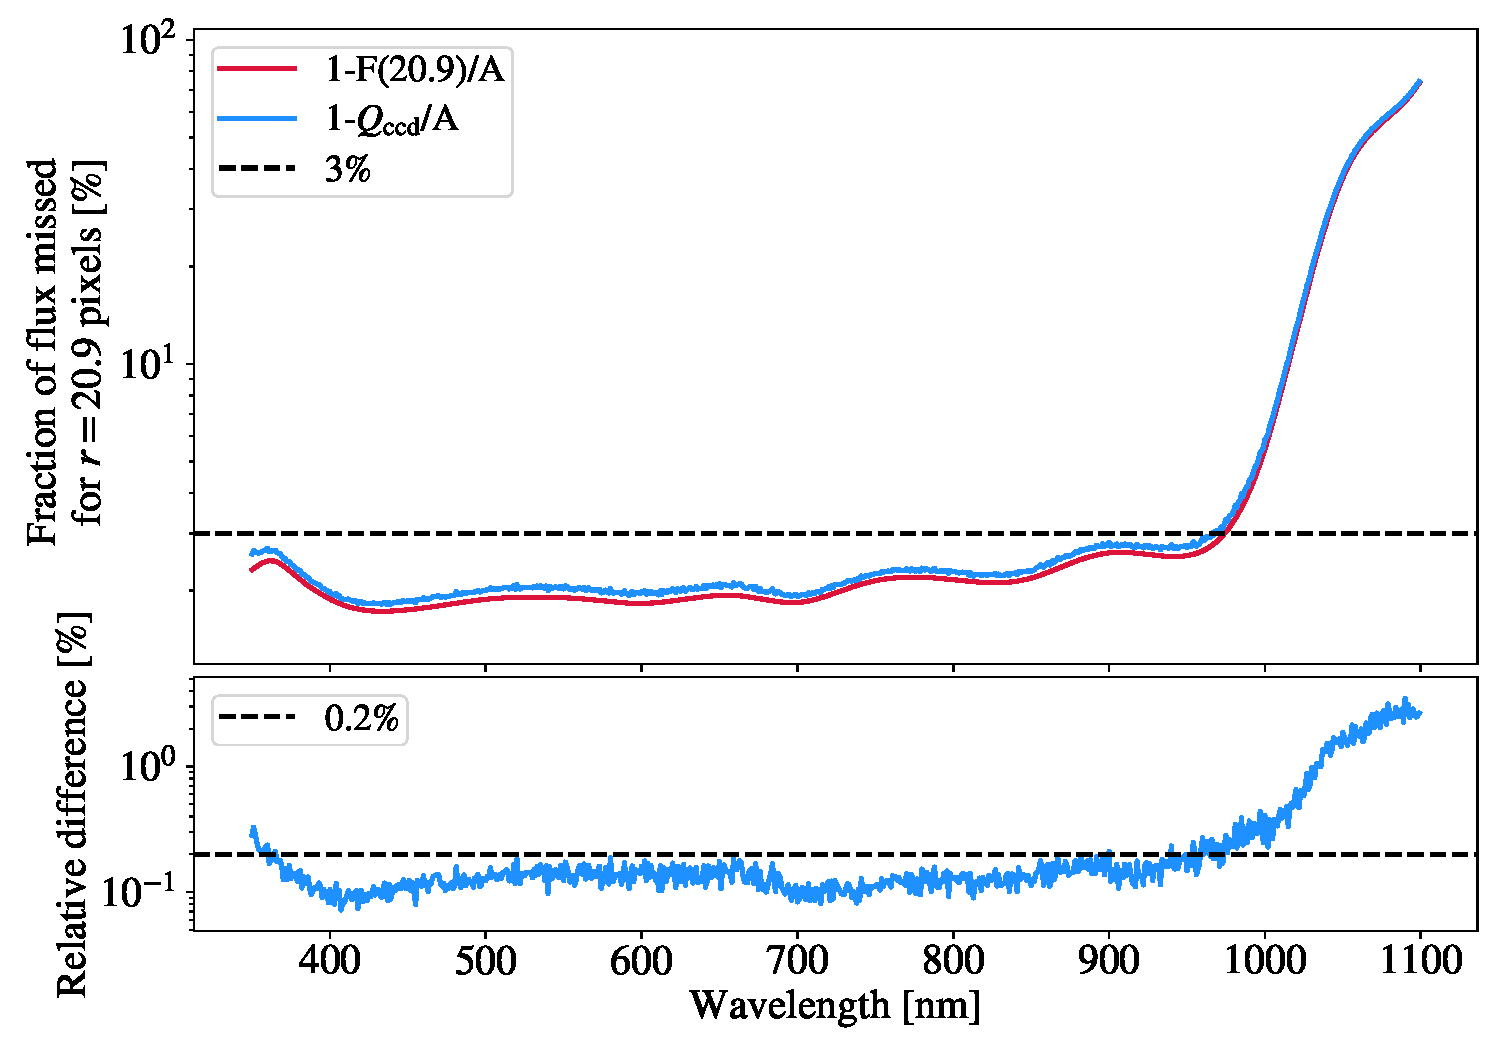
\includegraphics{fig/bias_aperture.pdf}}
     \caption{Top: Fraction of flux missed in percent against $\lambda_L$ when measuring \spinhole pinhole dataset with aperture photometry at \SI{20.9}{pixels} rather than taking the total amplitude $A$ fitted. The red curve corresponds to the estimation of the fit, the green one to aperture photometry when the backgruond is estimate with the dark datasets, and the blue one to aperture photometry when the background is estimate with the method described in Section~\ref{sec:photometry}. Bottom: Relative difference in percent between the flux measured for aperture photometry with the two background estimations and the model estimation at \SI{20.9}{pixels}.}
     \label{fig:bias_aperture}
    %~/stardice/analysis/cbp_paper/total_fluxes/ratio_pinholes.ipynb
\end{figure}

\subsection{Pinholes intercalibration}

We aim to measure the difference of \SD responses between the \spinhole pinhole and the \bpinhole pinhole. We want to measure the fluxes of the two responses with aperture photometry at the same radius and does not have any other consideration than the geometry of the pinholes. To do so, we estimate the \spinhole pinhole flux $F(300)$ with the model from Equation~\ref{eq:moffat_model}. We compute the ratio $\Kpinholes=\frac{F(300)}{\phi^{\bpinhole}_{300.00}}$ shown in Figure~\ref{fig:ratio_pinholes}. The linear fit of this ratio is used to intercalibrate the \bpinhole pinhole \SD response with the \spinhole pinhole \SD response. The slope is non-null and not expected as the ratio between the two pinholes should corresponds only to the ratio of surfaces of illuminated area at the input CBP. We suspect that some light diffusion on the edges of the pinholes or other complex reflections in the setup could give this ratio a chromatic dependance.

\begin{figure}[h]
    \centering
    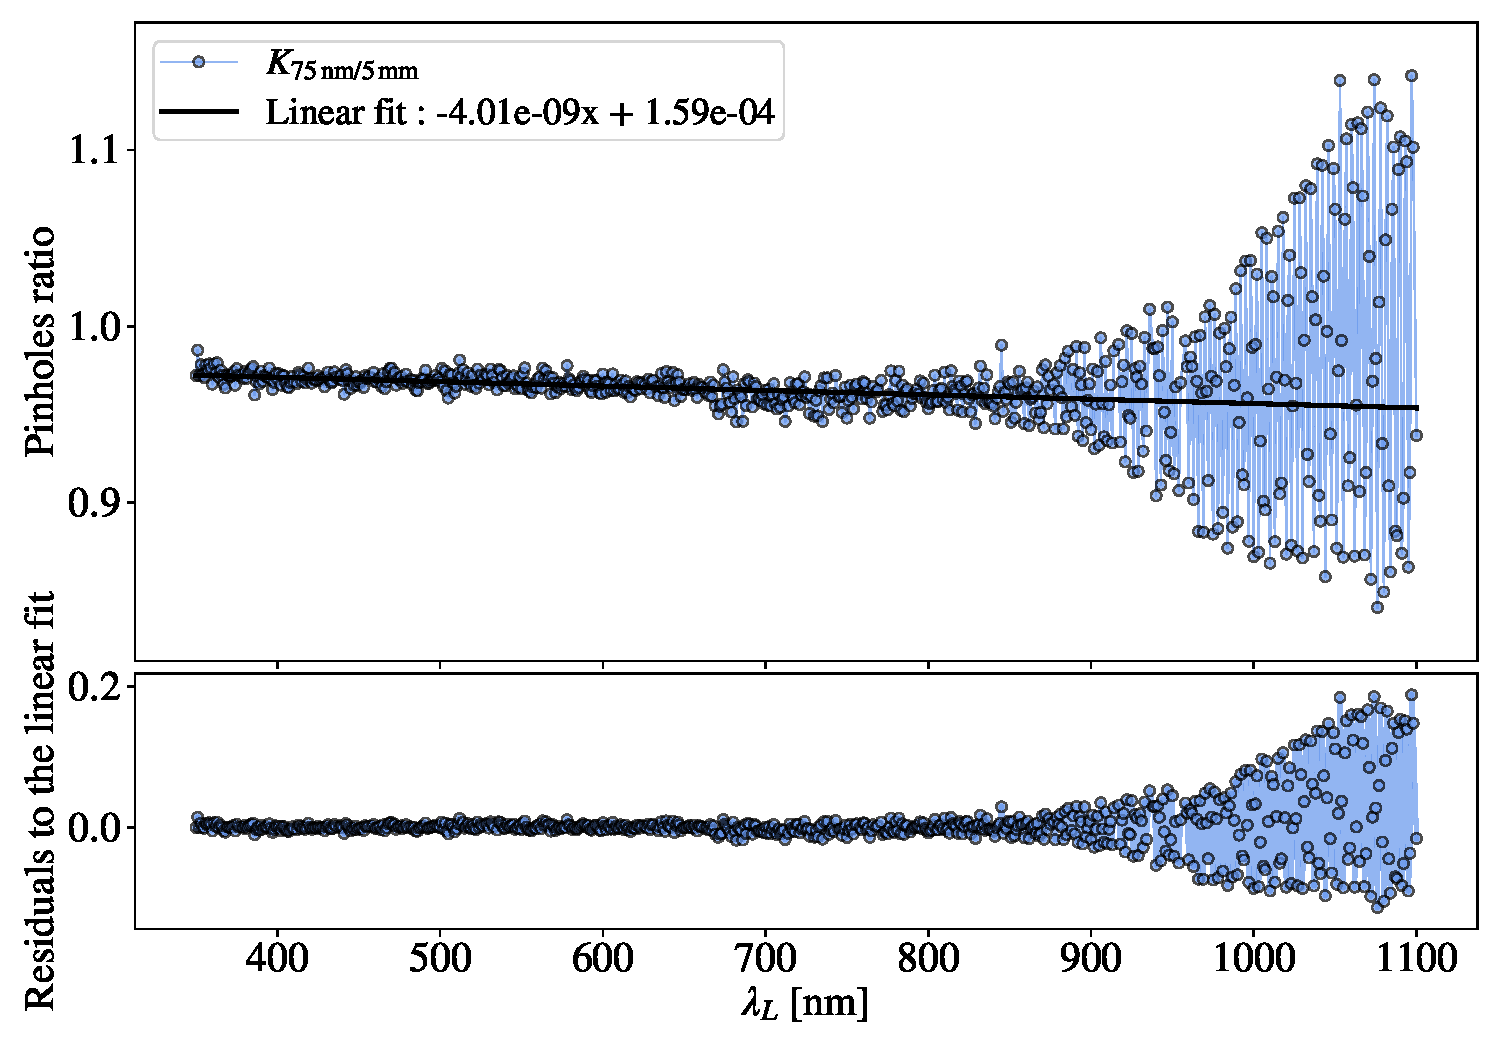
\includegraphics[width=\columnwidth]{fig/ratio_pinholes.pdf}
    \caption{Ratio $\Kpinholes$ with respect to wavelength. The black line corresponds to a linear fit between \SI{400}{\nm} and \SI{900}{\nm}.}
    \label{fig:ratio_pinholes}
    %~/stardice/analysis/cbp_paper/golden_sample_analysis/dr2/ratio_pinholes.ipynb
\end{figure}

% The bottom panel corresponds to the aperture correction that is needed to apply to the aperture photometry measurement. It is around 2\% below \SI{950}{\nano\meter}, and increase by one order of magnitude in the infrared. This increase is correlated with the variation of the Moffat parameters $\alpha$ and $\beta$, showing that the PSF is drastically changing in the near infrared. This issue is discussed in more details section \ref{sec:ir}. The third panel show a constant background against wavelength, at a mean of \SI{0.27}{ADU/pixel}.

%\subsection{Correction of the ghost contamination}
%\label{sec:ghost}
%
%In Section~\ref{sec:strategy} we discussed the need to intercalibrate the CBP response for both pinhole sizes. To this purpose, we took measurements with the \SD telescope with both \bpinhole pinhole and \spinhole pinhole, and evaluate the systematic related to this change of pinhole diameter. One major difference between the \spinhole pinhole and the \bpinhole pinhole is how the ghost and the main spot superimpose on the focal plane. We show in Figure~\ref{fig:schema_ghost} the optical path that produces the 1\up{st} order ghost on the focal plane. In Figure~\ref{fig:ghost_contrast}, we can see an image of the 1\up{st} order ghost next to the main spot obtained with the \spinhole pinhole. The distance between the centroïd of the main spot and the centroïd of the 1\up{st} order ghost is between 30 to 70 pixels depending on the radial position on the mirror. In the mean time, the \bpinhole pinhole photometry is made with an aperture of 300 pixels, containing the 1\up{st} order ghost and the main spot. We need to know the fraction of the flux that corresponds to the 1\up{st} order ghost.
%
%
%\subsubsection{First order ghost photometry}
%
%We want to quantify the contribution of the ghost relatively to the main spot for the \bpinhole pinhole. Let be $G_0(\lambda)$ the quantity of light collected in the main spot, and $G_\mathrm{n}(\lambda)$ the quantity of light collected in the ghost of order $n$. We define $\Kghost(\lambda)$ the ratio of the 1\up{st} order ghost $G_1(\lambda)$ over the main spot $G_0(\lambda)$:
%
%\begin{equation}
%    \Kghost = \frac{G_1(\lambda)}{G_0(\lambda)}.
%    \label{eq:ratio_ghost}
%\end{equation}
%We make the hypothesis that the ratio $\Kghost(\lambda)$ is the same for both pinholes. We measure $G_1(\lambda)$ with the \spinhole pinhole where it is well separated from $G_0(\lambda)$. We build a mask with the expected ghost shape and we fit its best position on the image. $G_1(\lambda)$ is the sum of the ADUs contained in this mask, after background subtraction. To estimate the background at this position, we assume that the main spot has a spatial vertical symmetry. We place a symmetric mask at the vertical symmetric position and measure the ADUs contained inside, which correspond to background only. This background is subtracted to the photometry of the 1\up{st} order ghost to obtain $G_1(\lambda)$. On the other hand, $G_0(\lambda)$ is measured with the aperture photometry described in \ref{sec:photometry}. 
%
% \begin{figure}[h]
%     \centering
%     \resizebox{\hsize}{!}{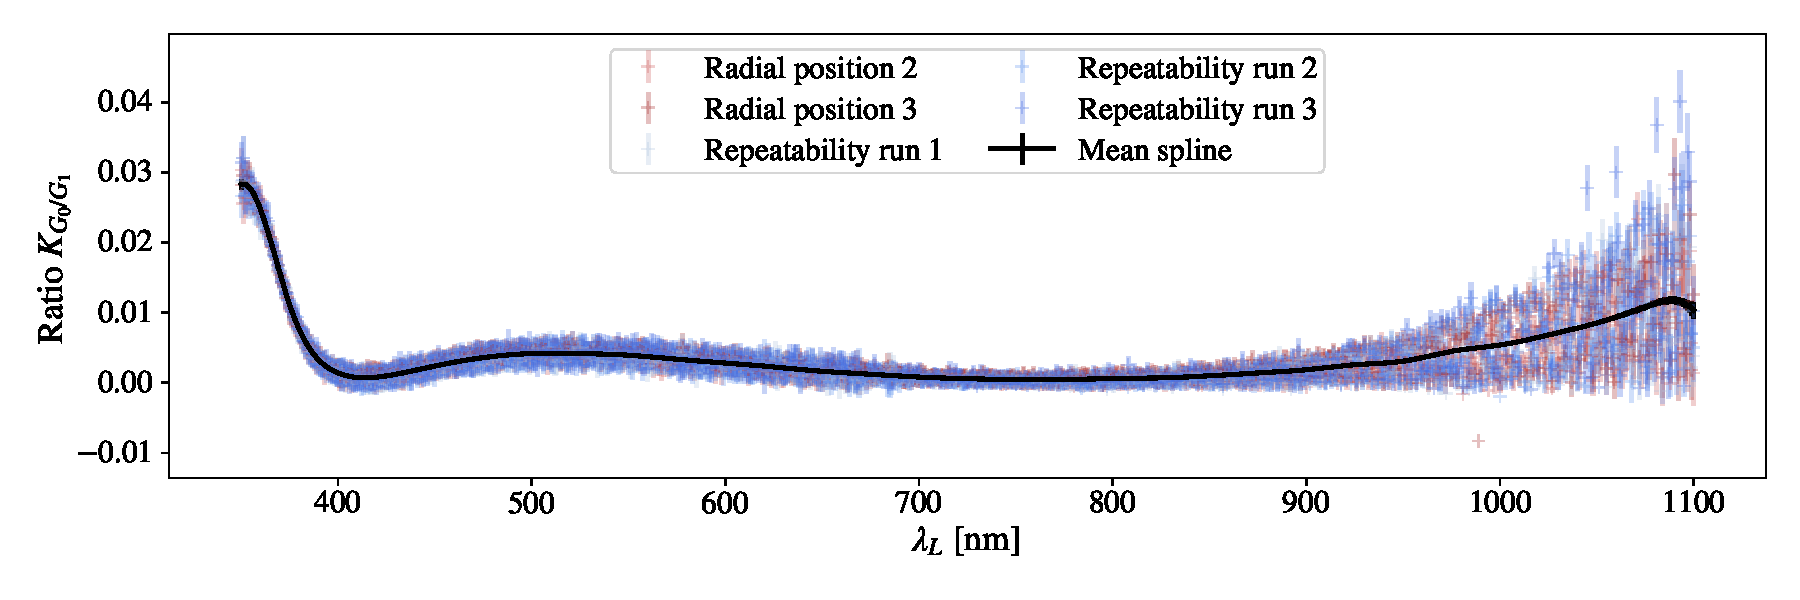
\includegraphics{fig/ghost_ratio.pdf}}
%     \caption{Ratio $\Kghost$ (which correspond to the order 1 ghost $G_{1}(\lambda)$ over the main spot $G_0(\lambda)$) with respect to $\lambda_L$. The mean spline goes through five datasets, three at the same position on the mirror, two other at a different radial position on the mirror. All responses are at the same position on the focal plane.}
%     \label{fig:ghost_ratio}
%    %~/stardice/analysis/cbp_paper/golden_sample_analysis/dr2/ghost_photometry_general.ipynb
% \end{figure}
% 
% 
% 
% \subsubsection{Contribution of the n\up{th} order ghosts}
%
%Now that we did the photometry for the first order ghost, we want to estimate the contribution of higher orders. Since the intensity of these ghosts is very weak and hard to analyse, we simulate their contribution from the $1^{\mathrm{st}}$ order ghost analysis. Let be $\Rwindow$ the reflection coefficient at the interface air-window, and $\Rccd$ the reflection coefficient at the interface air-CCD. We know the transmission of the window $T_\mathrm{window}(\lambda)$ from manufacturer datasheets, so we can infer $\Rwindow$:
% 
%\begin{equation}
%    \Rwindow = 1 - T_\mathrm{window}(\lambda).
%    \label{eq:rwindow}
%\end{equation}
% 
%\noindent We define $F$ the flux collected by the camera, $G_0(\lambda)$ the quantity of light collected in the main spot, and $G_\mathrm{n}(\lambda)$ the quantity of light collected in the ghost of order $n$. $G_0(\lambda)$ and $G_\mathrm{n}(\lambda)$ are a function of F: 
%
%\begin{equation}
%     G_0(\lambda) = (1-\Rwindow)^{2} \times (1-\Rccd) \times F, 
%     \label{eq:g0}
%\end{equation}
%
%\begin{equation}
%\begin{aligned}
%    G_\mathrm{n}(\lambda) & = G_{0}(\lambda) \times [\Rccd \Rwindow + \Rccd(1-\Rwindow)\Rwindow]^{n} \\
%    & = G_{0}(\lambda) \times [2 \Rccd \Rwindow - \Rccd \Rwindow^{2}] ^{n}. \\
%     \label{eq:gn}
%\end{aligned}
%\end{equation}
%
%\noindent The sum of all the ghosts $G_{\mathrm{n>0}}(\lambda)$ is defined as
%\footnote{If |q| < 1, the serie $\left( \sum_{n=0}^{m} q^n \right)_{\mathrm{m \in \mathbb{N}}}$ strictly converge and \\ $\sum_{n=0}^{\infty} q^n \equiv \lim\limits_{m \rightarrow \infty} \sum_{n=0}^{m} q^n = \frac{1}{1-q}$}:
%
% \begin{equation}
% \begin{aligned}
%     G_{n>0}(\lambda)&=\sum_{n=0}^{\mathrm{n} \rightarrow \infty} G_\mathrm{n}(\lambda) - G_0(\lambda) \\
%     & = G_0(\lambda) \times \sum_{n=0}^{n \rightarrow \infty} \left( [2 \Rccd \Rwindow - \Rccd \Rwindow^{2}] ^{n} - G_0(\lambda) \right)\\
%     & = G_0(\lambda) \times\left( \frac{1}{1- [2 \Rccd \Rwindow - \Rccd \Rwindow^{2}]} - 1\right),
%     \label{eq:sum_ghost}
% \end{aligned}
% \end{equation}
% 
%\noindent and the sum of the ghost of order higher than 1 is defined as:
%
% \begin{equation}
%     G_{n>1}(\lambda) = G_{n>0}(\lambda) - G_1(\lambda).
%     \label{eq:sum_ghost_sup_1}
% \end{equation}
%
%\noindent As we measure the photometry of the 1\up{st} order ghost $G_1(\lambda)$, we want to verify that the ghosts of higher orders $G_{\mathrm{n}>1}(\lambda)$ are negligible. Using the Equations~\ref{eq:ratio_ghost}, \ref{eq:g0} and \ref{eq:gn}, we can compute $\Rccd$:
%
%\begin{equation}
%    \Rccd = \frac{\Kghost}{\Rwindow (2 - \Rwindow)}.
%    \label{eq:rccd}
%\end{equation}
%
%We measured $G_1(\lambda)$ with photometry, and estimate $G_{\mathrm{n}>1}$ with the equations above. We show the ratio $K_{G_{\mathrm{n}>1}/G_0}$ in Figure~\ref{fig:ratio_ginf_g0}, and we see that $K_{G_{\mathrm{n}>1}/G_0}$ is always below the per mil level. Since $G_{\mathrm{n}>1}$ contribute for less than a per mil of $G_0(\lambda)$, we decide to neglect it.
%
%\begin{figure}[h]
%    \centering
%    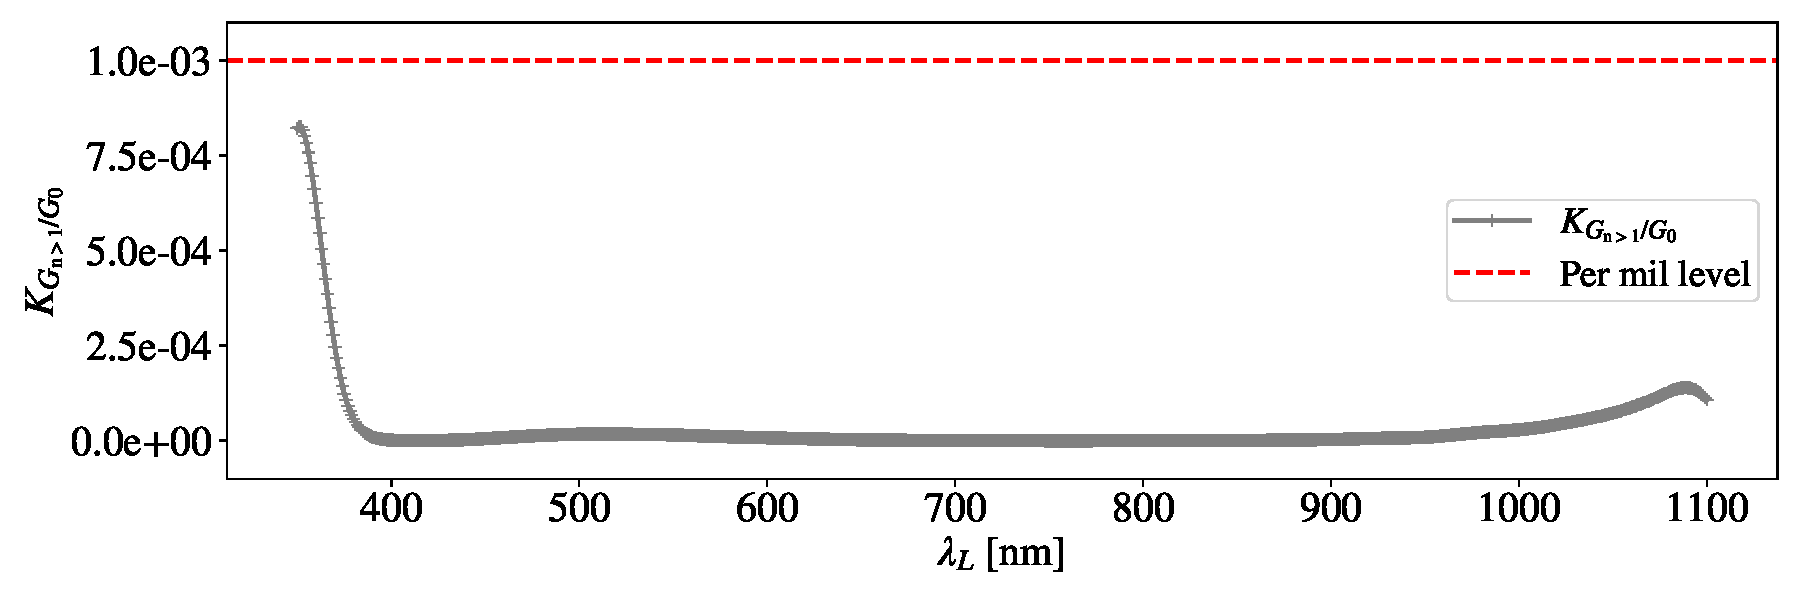
\includegraphics[width=\columnwidth]{fig/ratio_g1_ginf.pdf}
%    \caption{Ratio $K_{G_{\mathrm{n}>1}/G_0}(\lambda)$ (which correspond to the sum of the ghosts at order higher than 1 $G_{\mathrm{n}>1}(\lambda)$ over $G_0(\lambda)$) with respect to $\lambda_L$.}
%    \label{fig:ratio_ginf_g0}
%    %~/stardice/analysis/cbp_paper/golden_sample_analysis/dr2/ghost_convergence.ipynb   
%\end{figure}

%\subsubsection{Ghost contribution for \bpinhole pinhole}
%
%The total charges $\Qccd{}_{, \, \SI{5}{\milli\meter}}(\lambda)$ measured by doing the aperture photometry at 300 pixels for the \bpinhole pinhole is the sum of the charges $Q_0(\lambda)$ in the main spot $G_0(\lambda)$ and the charges $\Qghost(\lambda)$ in the 1\up{st} order ghost $G_1(\lambda)$. With $\Eccd$ the quantum efficiency of the StarDICE CCD camera, we define these quantites as:
%
%\begin{equation}
%    \Qghost(\lambda) = G_1(\lambda) \times \Eccd, 
%    \label{eq:qghost}
%\end{equation}
%
%\begin{equation}
%    Q_0(\lambda) = G_0(\lambda) \times \Eccd.
%    \label{eq:qmain}
%\end{equation}
%
%\noindent Then $Q_0(\lambda)$ can be measured as follow:
%
%\begin{equation}
%\begin{aligned}
%    Q_0(\lambda) & = \Qccd{}_{, \, \SI{5}{\milli\meter}}(\lambda) - \Qghost(\lambda) \\
%    & = \frac{\Qccd{}_{, \, \SI{5}{\milli\meter}}(\lambda)}{1 + \Kghost}.
%    \label{eq:qccd_5mm}
%\end{aligned}
%\end{equation}
%We use the estimation of $\Kghost$ with the \spinhole pinhole to obtain $Q_0(\lambda)$. 
%
%\noindent Once we have corrected the \bpinhole pinhole from the ghost contribution, we can compute the ratio between the \SD responses defined as $\Kpinholes$: 
%\begin{equation}
%    \Kpinholes = \frac{\Rcbp^{\bpinhole}(\lambda)}{\Rcbp^{\spinhole}(\lambda)}.
%    \label{eq:ratio_pinholes}
%\end{equation}
%Thanks to this equation, we can infer $\Rcbp^{\spinhole}(\lambda)$ from the measurement of $\Rcbp^{\bpinhole}(\lambda)$.
%
%\THIERRY{à finir : comment on corrige le ghost ? est-ce que la correction d'ouverture est suffisante ?}
%
%We show these ratios before and after the ghost correction in the upper Figure~\ref{fig:ratio_pinholes}. We expect the ratio to be linear since it should be the ratio of two surfaces, so we draw a linear spline through the data. In the ultraviolet below \SI{400}{\nm} where the window is highly reflective, we see that the ghost correction has flattened the ratios. Above \SI{900}{\nm} we can see a significative difference between the ratio and the linear spline. This phenomenon is not quite understood and is discussed in section \ref{sec:discussion}, but we precise that the linear fit is made only for the wavelengths below \SI{900}{\nano\meter}. 
%
%\begin{figure}[h]
%    \centering
%    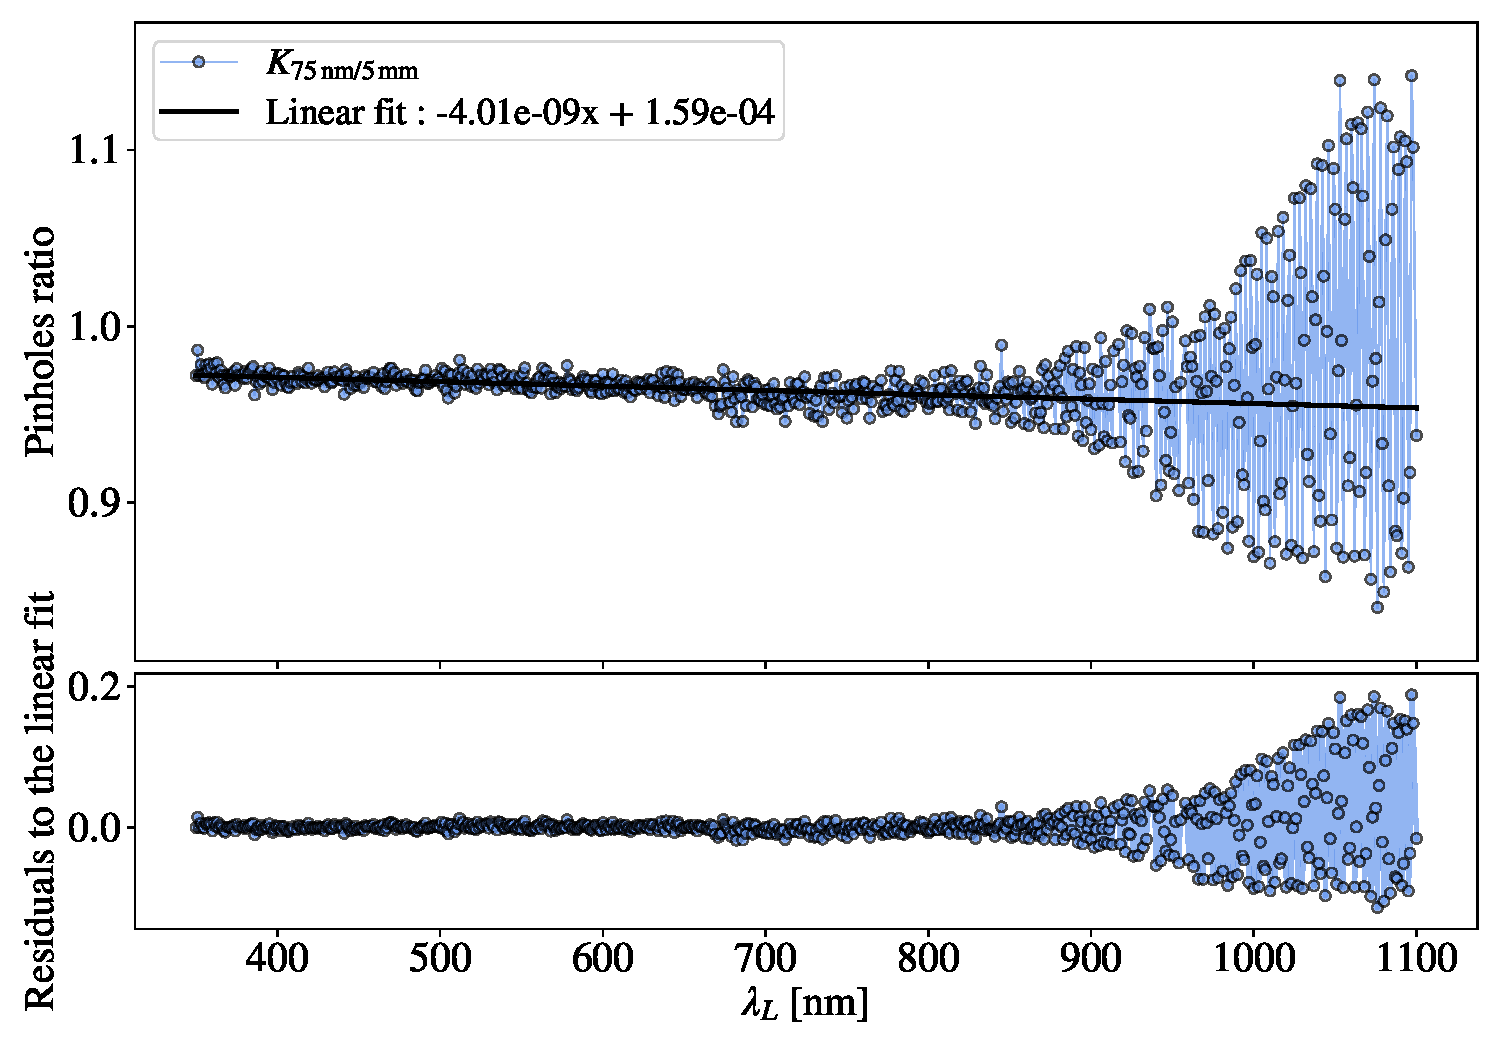
\includegraphics[width=\columnwidth]{fig/ratio_pinholes.pdf}
%    \caption{Ratio $\Kpinholes(\lambda)$ with respect to wavelength, before and after ghost correction. We compute a linear spline that best fit the data between \SI{400}{\nm} and \SI{900}{\nm}.}
%    \label{fig:ratio_pinholes}
%    %~/stardice/analysis/cbp_paper/golden_sample_analysis/dr2/ratio_pinholes.ipynb
%\end{figure}
%
%\subsubsection{Summary}
%
%The summary of the error budget on the \SD telescope response id detailed in Figure~\ref{fig:sd_budget}
%
%
%\begin{figure}
%    \centering
%    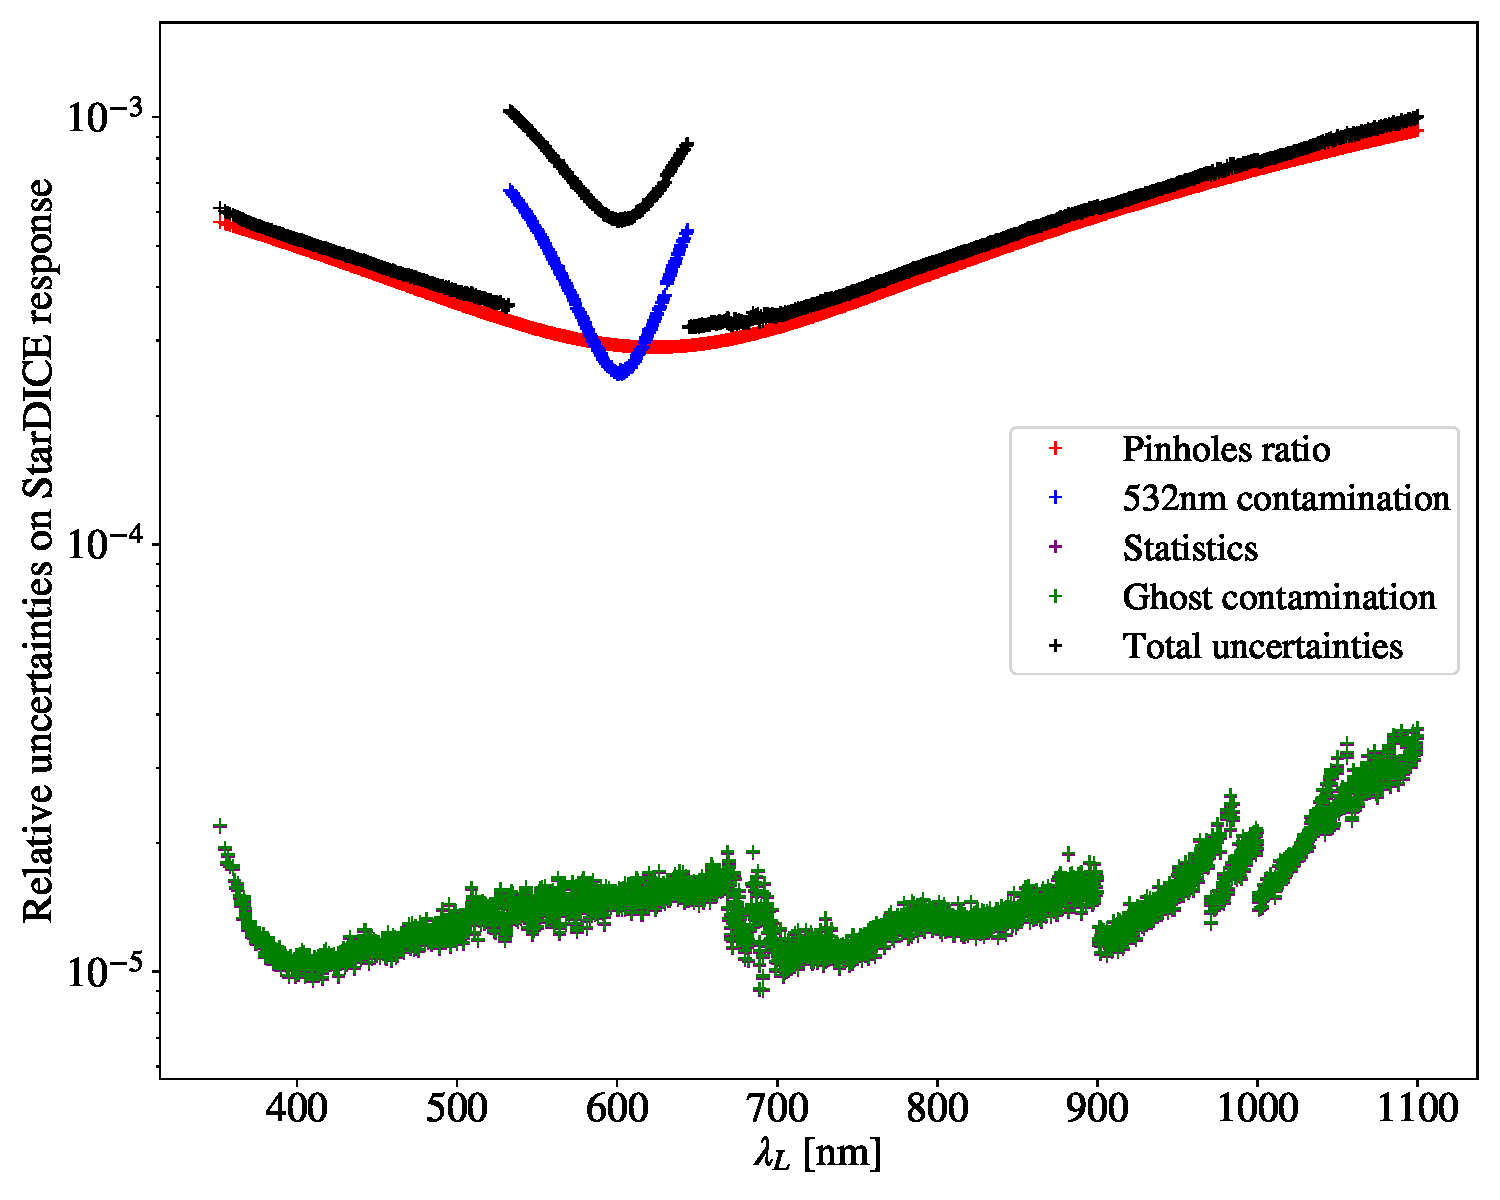
\includegraphics[width=\columnwidth]{fig/sd_uncertainties_budget.pdf}
%    \caption{Total error budget for \SD response.}
%    \label{fig:sd_budget}
%\end{figure}

\subsection{Correction of the light contamination}\label{sec:sd_contaminations}

When extracting the charges from the \SD camera, we have to remove light contaminations described in Sections~\ref{sec:532_cont} and~\ref{sec:fluorescence}. As the photodiode and the solar cell, the total charge measured in the \SD camera $\Qccdmes$ is the sum of the charges from the main laser line $\Qccdcal$ and the charges from the \SI{532}{\nm} contamination $\Qccd^{532}$, the $\lambda_{\rm comp}$ contamination $\Qccd^{\lambda_{\rm comp}}$, and the integrating sphere fluorescence $\Qccd^{\mathrm{fluo}}$, as follows:
\begin{equation}
    \Qccdmes = \Qccdcal + \Qccd^{532} + \Qccd^{\lambda_{\rm comp}} + \Qccd^{\mathrm{fluo}}
    \label{eq:qccd_mes}
\end{equation}
As we defined the final calibrated amount of charges detected in the solar cell $\Qsolarcal$, we do the same with the \SD CCD. The light detected by the \SD CCD has gone through the CBP optics and the \SD telescope. These instruments have respectively optical responses defined as $\Rcbp(\lambda)$ and $\Rtel(\lambda)$. We can define $R(\lambda)$ the total response of the CBP and the \SD telescope optics:
\begin{equation}
    R(\lambda) = \Rtel(\lambda) \times \Rcbp(\lambda).
    \label{eq:rtot}
\end{equation}
Then, the contamination contribution in \SD camera from every source is evaluated multiplying photodiode charge contamination by $R(\lambda)$.
The impact of these subtractions is illutrated in Figure~\ref{fig:g_filter_532} focusing on the \SD g filter, the most affected filter by integrating sphere fluorescence and \SI{532}{\nano\meter} line.

\begin{figure}[h]
    \centering
    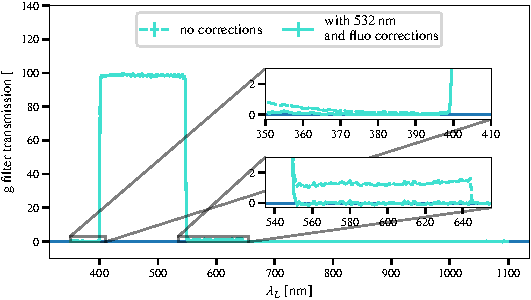
\includegraphics[width=\columnwidth]{fig/g_filter_532.pdf}
    \caption{\SD g filter transmission as a function of the set laser wavelength $\lambda_L$, with and without the \SI{532}{\nm} correction. For clarity, we added a zoom on the out-of-band transmission where $\SI{532}{\nm}$ line is transmitted while higher wavelengths are shot by the laser.}
    \label{fig:g_filter_532}
    %cbp_paper_plots.ipynb
\end{figure}

\subsection{\SD response scan}

\subsubsection{\SD optics, filters and grating responses}

In this section we present the results of our different measurements. The following measurements are all taken at the same position on the mirror and the focal plane. The Figure~\ref{fig:stardice_5mm_response} show the \SD response obtained with the \bpinhole pinhole, and no filter. The Figure~\ref{fig:stardice_75um_response} show the \SD response obtained with the \spinhole pinhole, with all filters. In this figure we have a wavelength resolution sufficient enough to see the filter edges. The Figure~\ref{fig:stardice_grating_response} show the \SD response obtained with the \spinhole pinhole, with the grating set in front of the camera. The grating being blazed so that the 1\up{st} order of diffraction is the brightest, so we will mainly focus on this order of diffraction. We see a cut of the 2\up{nd} and 3\up{rd} order that correspond to the wavelength at which the signal is outside the CCD sensor.

\begin{figure}[h]
    \centering
    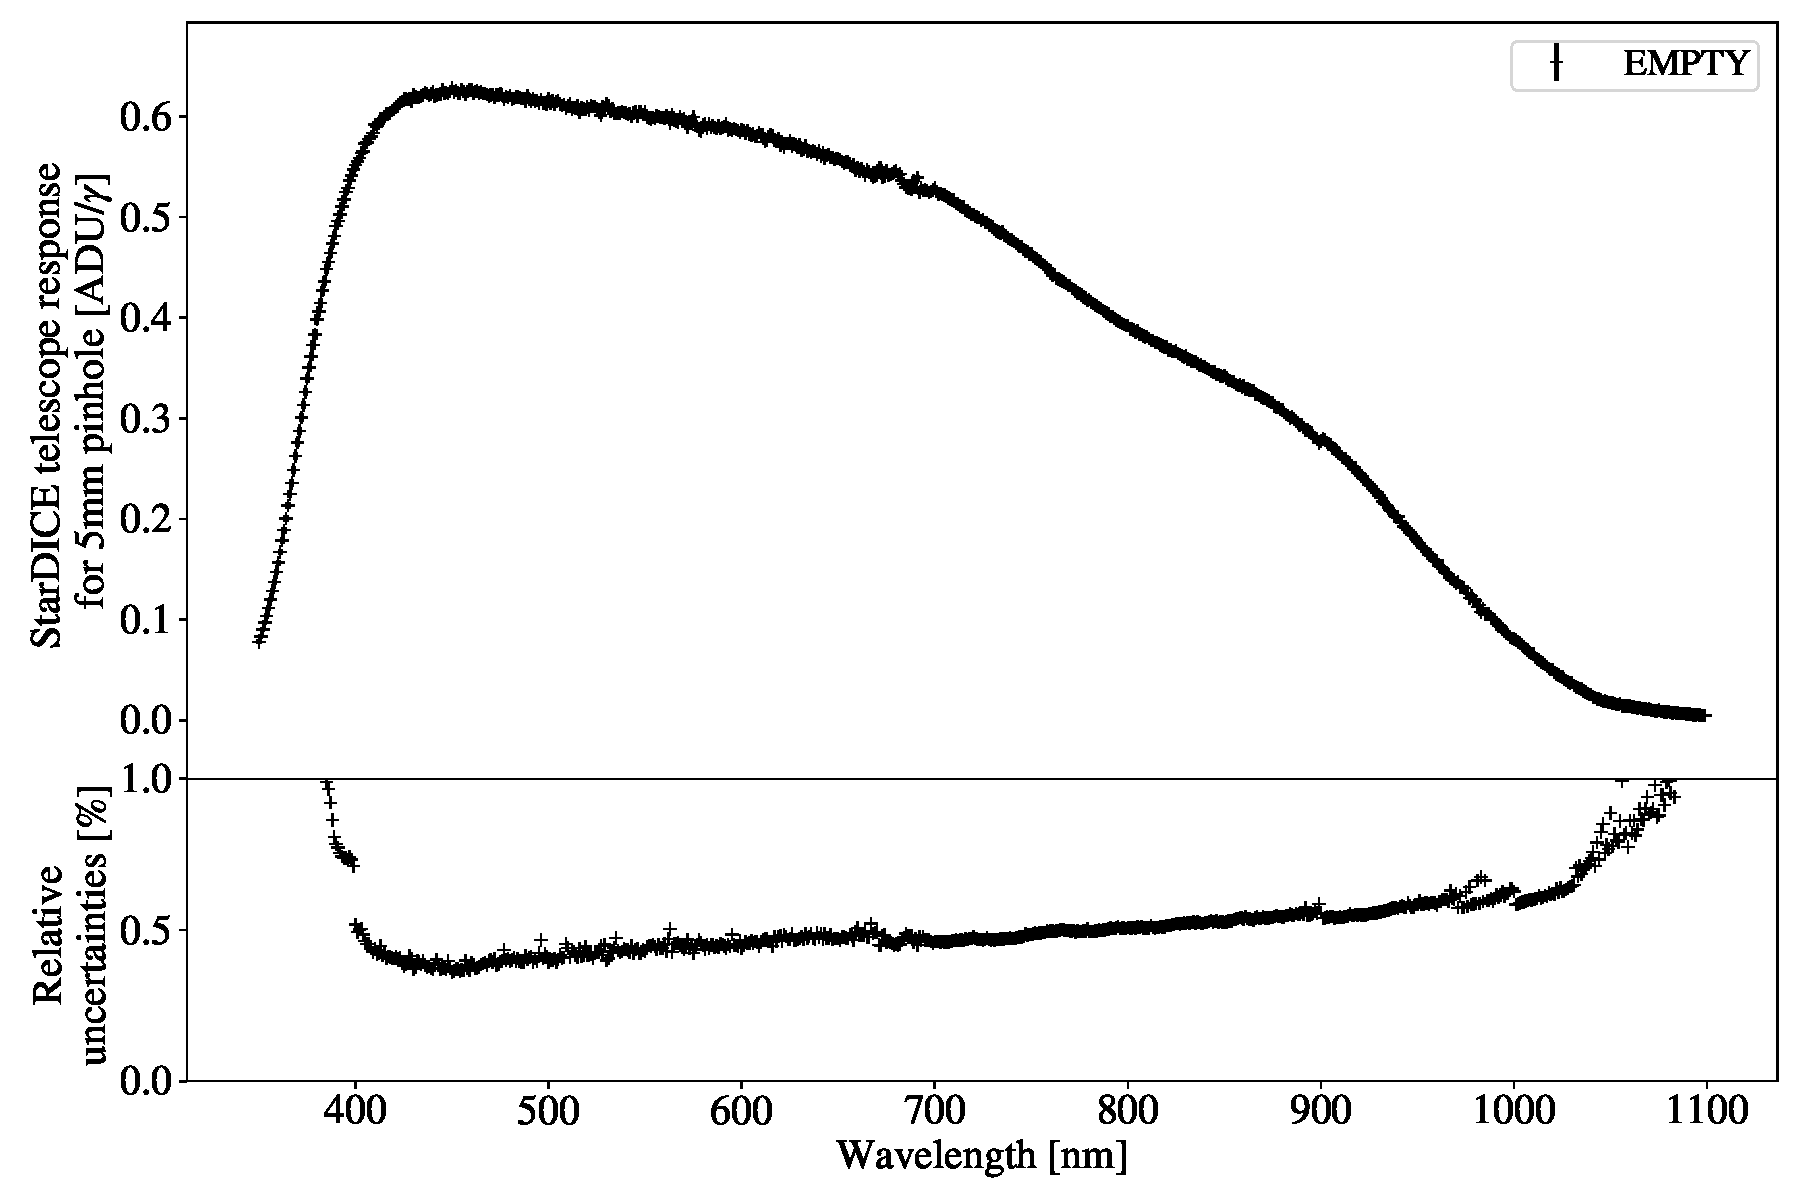
\includegraphics[width=\columnwidth]{fig/stardice_5mm_response.pdf}
    \caption{Up : \SD response with no filter and \bpinhole pinhole with respect to wavelength in nanometer. Bottom : Uncertainties over the \SD response measurement with respect to wavelength in nanometer.}
    \label{fig:stardice_5mm_response}
    %~/stardice/analysis/cbp_paper/golden_sample_analysis/dr2/response_plots.ipynb
\end{figure}

\begin{figure}[h]
    \centering
    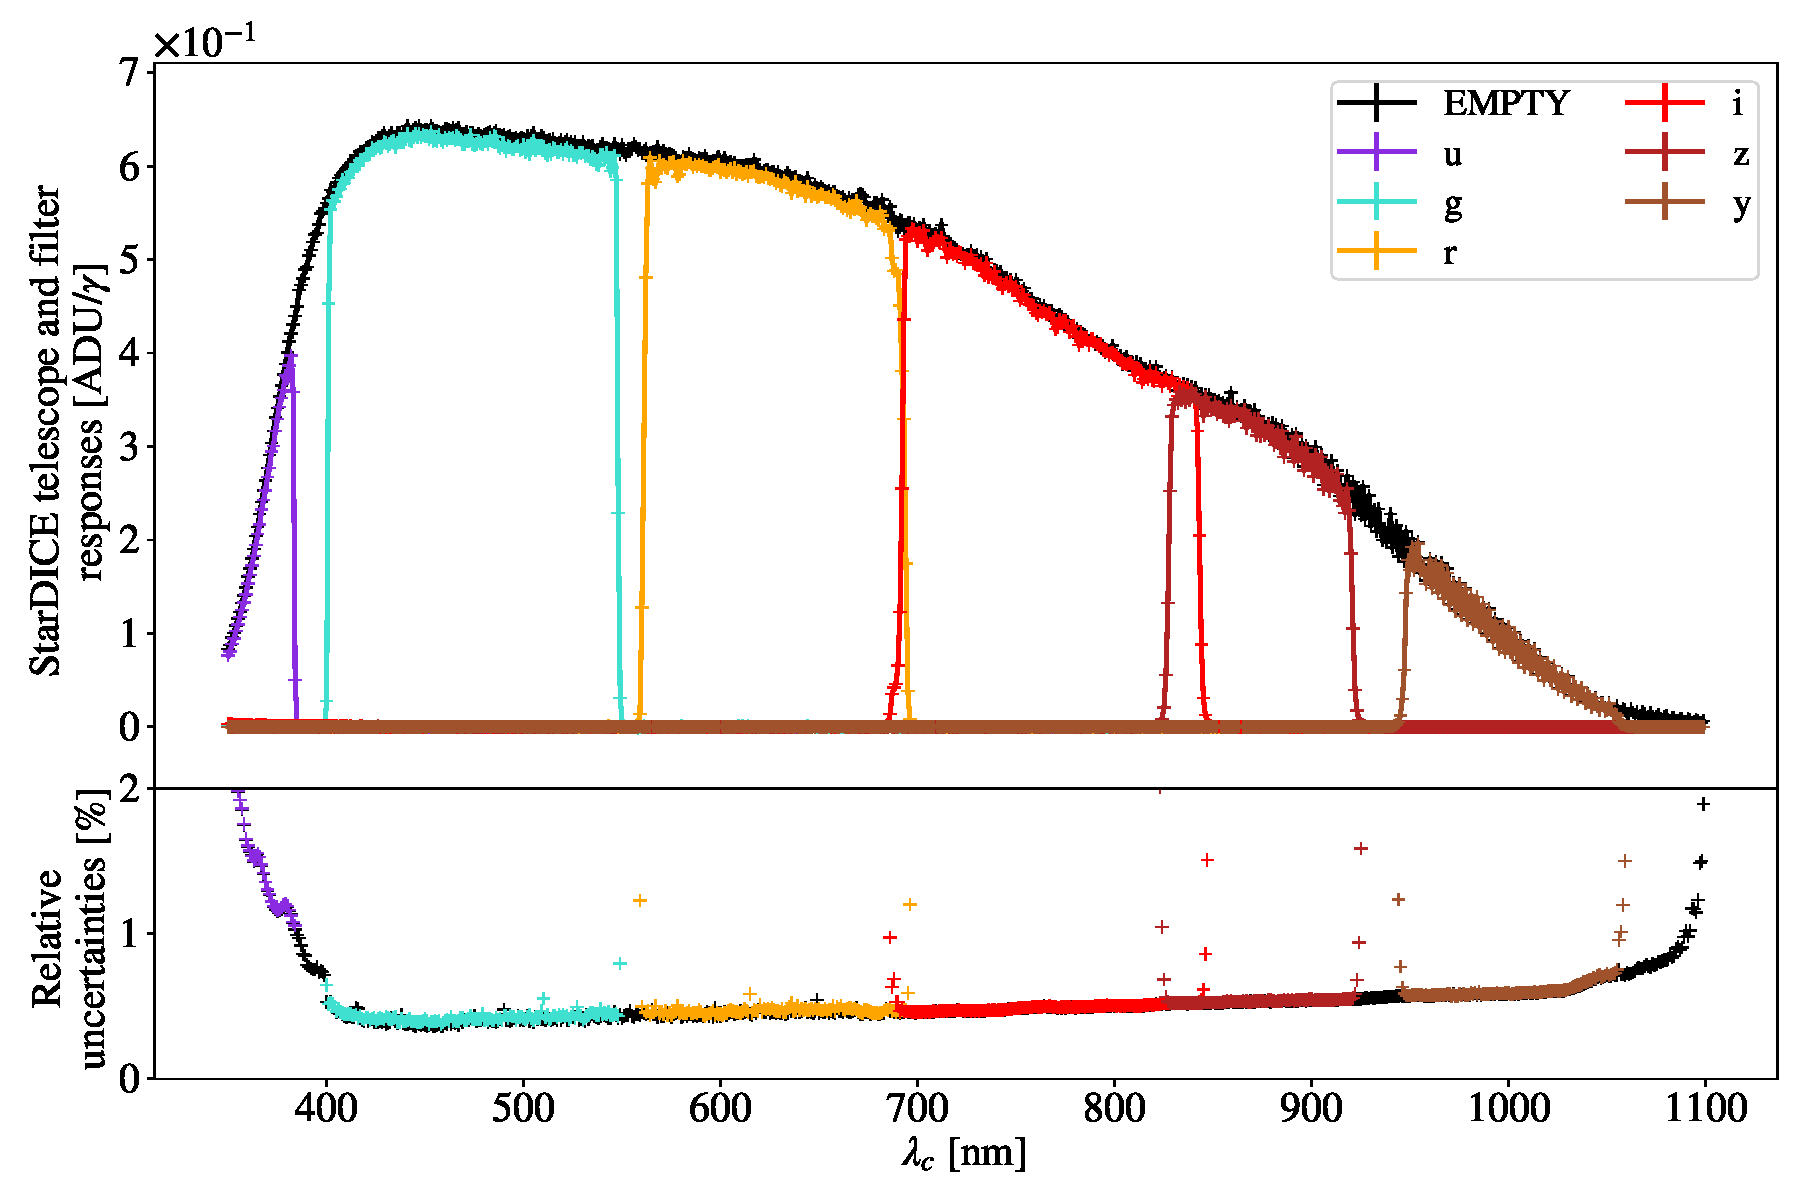
\includegraphics[width=\columnwidth]{fig/stardice_75um_response.pdf}
    \caption{Up : \SD response with at all filters and \spinhole pinhole with respect to wavelength in nanometer. Bottom : Uncertainties over the \SD response measurement with respect to wavelength in nanometer.}
    \label{fig:stardice_75um_response}
    %~/stardice/analysis/cbp_paper/golden_sample_analysis/dr2/response_plots.ipynb
\end{figure}

\begin{figure}[h]
    \centering
    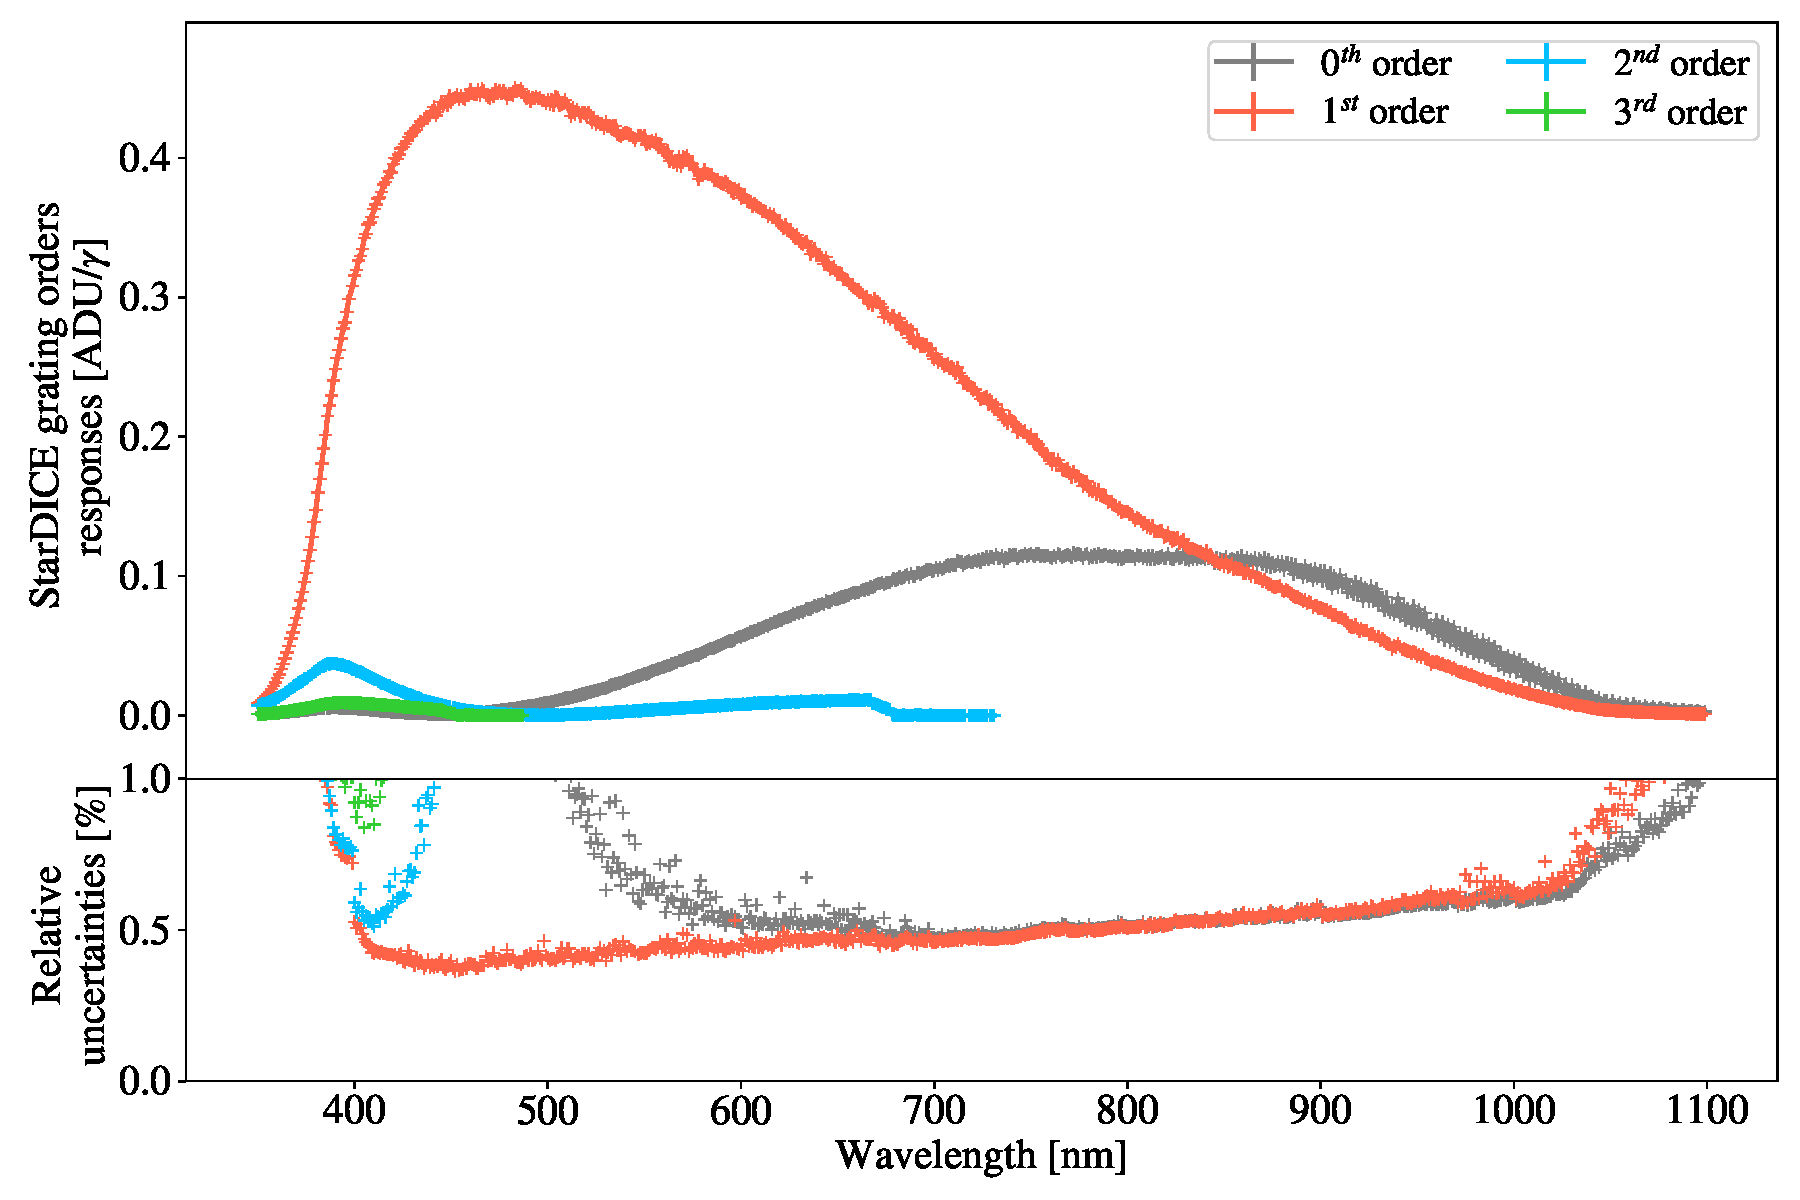
\includegraphics[width=\columnwidth]{fig/stardice_grating_response.pdf}
    \caption{Up : \SD response with the grating in front of the camera and \spinhole pinhole with respect to wavelength in nanometer. Bottom : Uncertainties over the \SD response measurement with respect to wavelength in nanometer.}
    \label{fig:stardice_grating_response}
    %~/stardice/analysis/cbp_paper/golden_sample_analysis/dr2/response_plots.ipynb
\end{figure}

\subsubsection{Radial positions}

The upper Figure~\ref{fig:radial_positions} show the \SD response obtained with the \spinhole pinhole and without filters for the different radial positions on the mirror shown in Figure~\ref{fig:8_mirror_positions} left, and the same focal plane position. The lower figure show the normalized residuals to the mean spline going through the four responses. In the ultraviolet below \SI{450}{\nm}, we can see a significant difference between the four radial positions. It goes up to 30\%, and it will be discussed in the section \ref{sec:discussion}. What we see above \SI{1000}{\nm} in the infrared is the result of the data oscillations around the spline caused by the fringing. 

\begin{figure}[h]
    \centering
    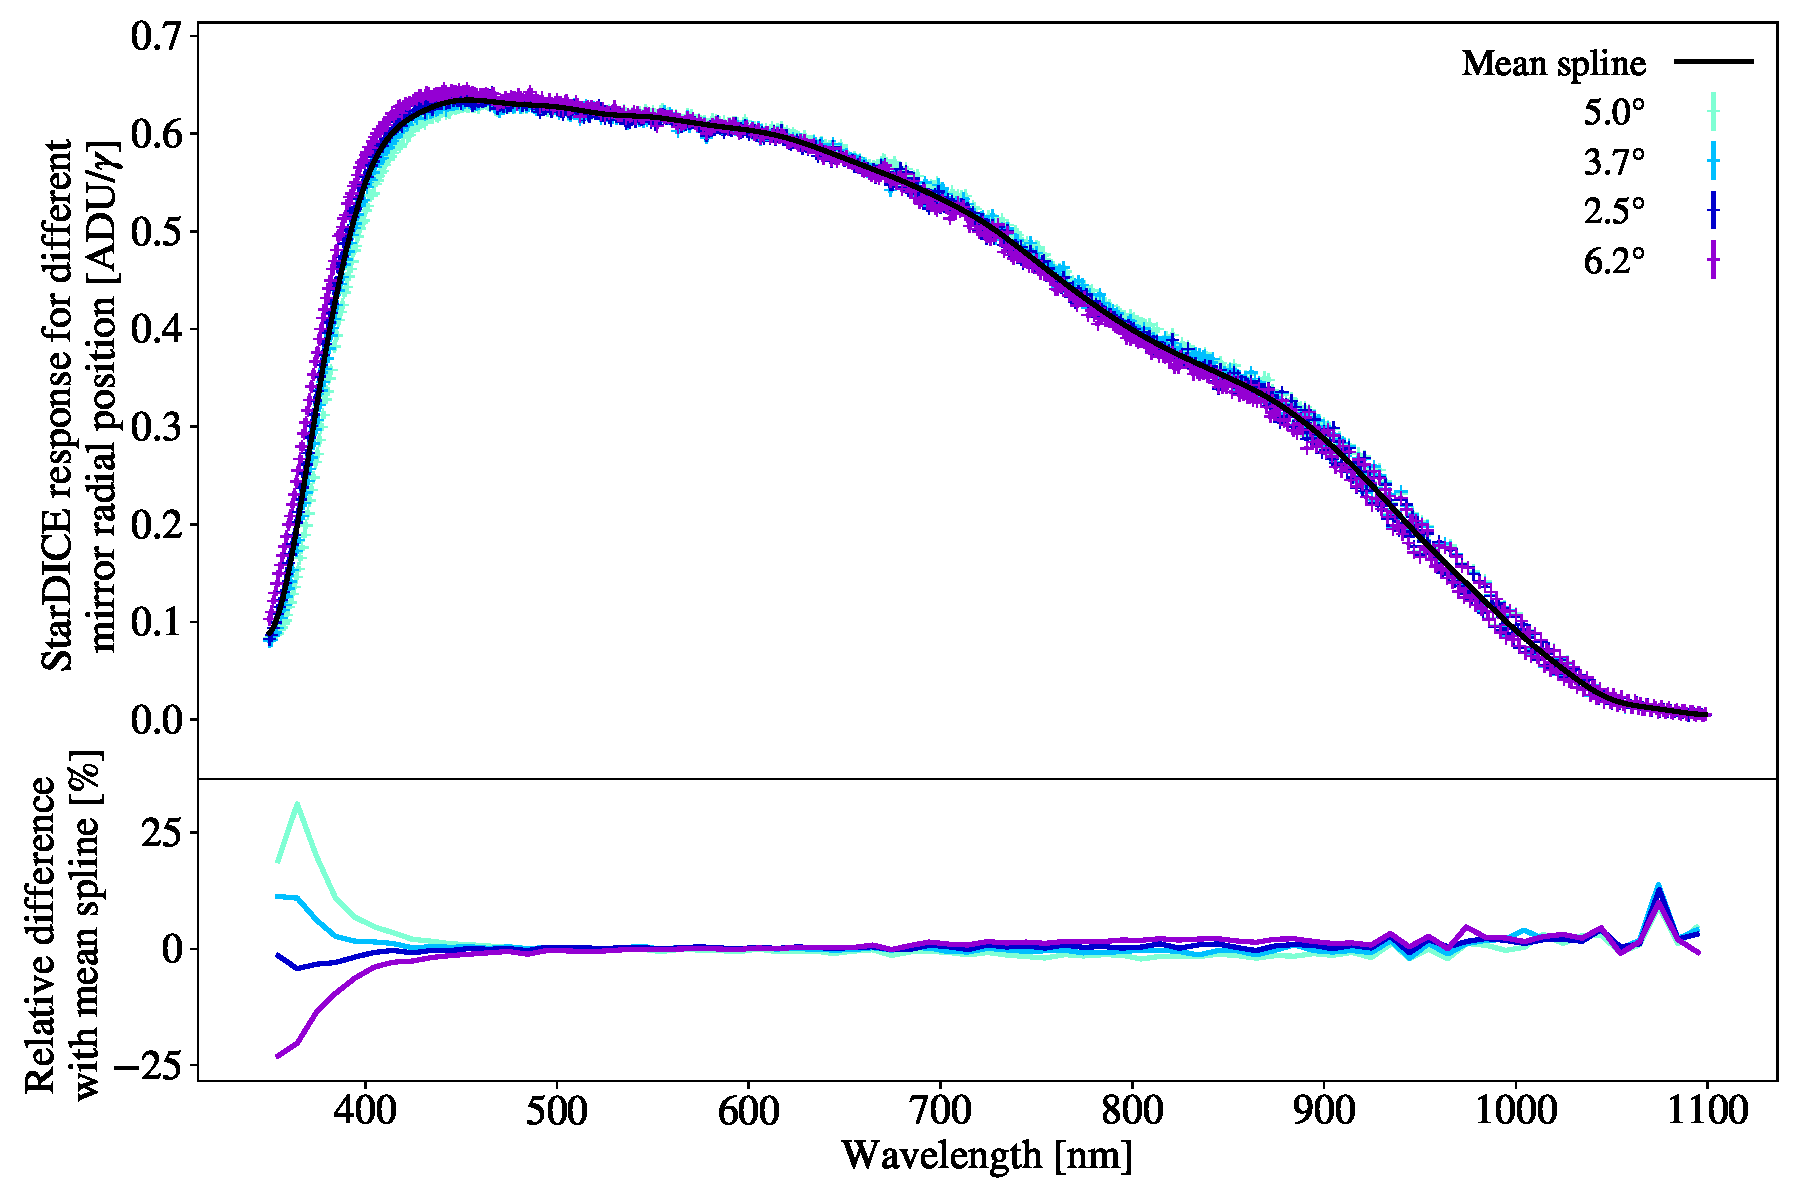
\includegraphics[width=\columnwidth]{fig/radial_positions.pdf}
    \caption{Top : \SD response for the different radial positions on the mirror, but same position on the focal plane. Bottom : Relative difference between the data and the mean spline.}
    \label{fig:radial_positions}
    %~/stardice/analysis/cbp_paper/golden_sample_analysis/dr2/2022_03_01_stardice_transmission_radius.ipynb
\end{figure}

\subsubsection{Quadrant positions}

The upper Figure~\ref{fig:radial_positions} show the \SD response obtained with the \spinhole pinhole and without filters for the different quadrant positions on the mirror shown in Figure~\ref{fig:8_mirror_positions} right, and the same focal plane position. The lower figure show the normalized residuals to the mean spline going through the four responses. We see again a divergence below \SI{400}{\nm} of about 20\% at most. The phenomenon in the infrared is still caused by the fringing. 

\begin{figure}[h]
    \centering
    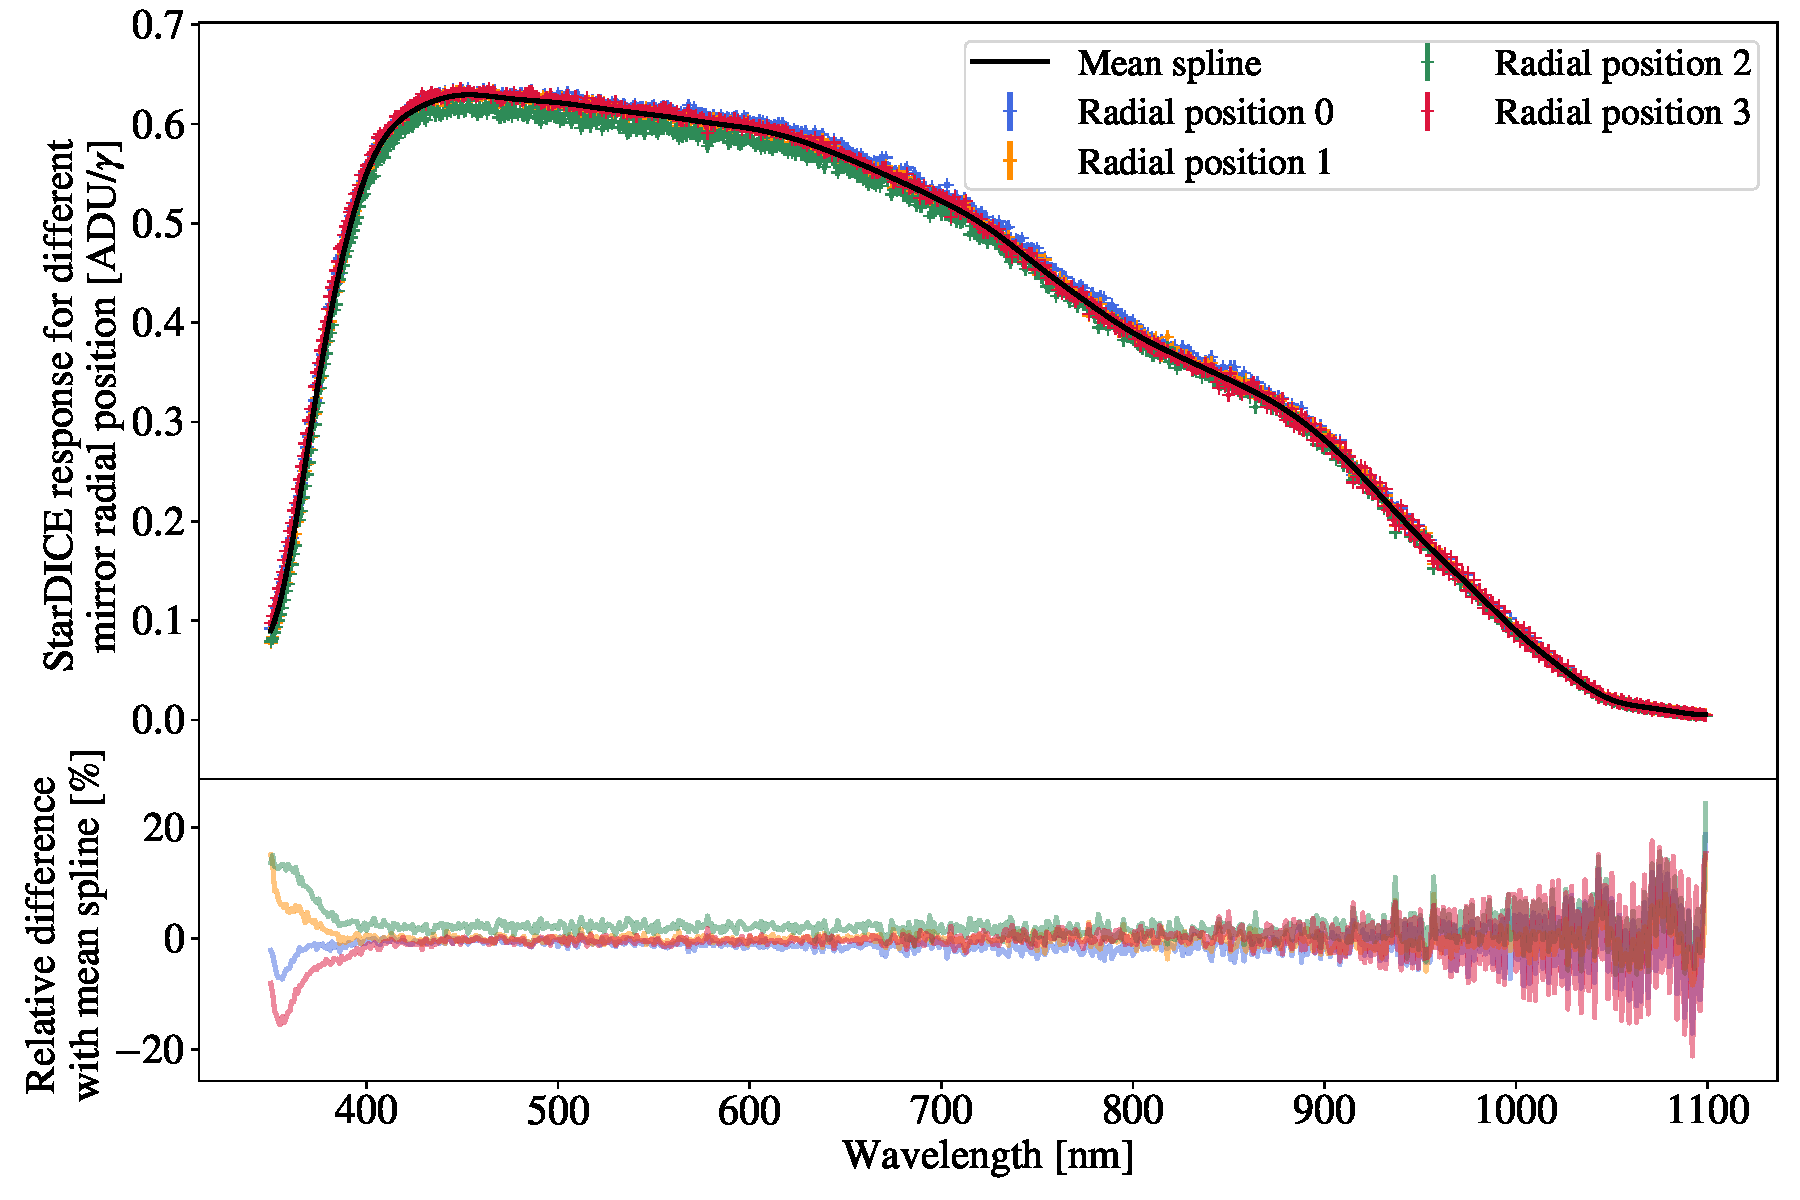
\includegraphics[width=\columnwidth]{fig/quadrant_positions.pdf}
    \caption{Top : \SD response for the different quadrant positions on the mirror, but same position on the focal plane. Bottom : Relative difference between the data and the mean spline.}
    \label{fig:quadrant_positions}
    %~/stardice/analysis/cbp_paper/golden_sample_analysis/dr2/2022_03_01_stardice_transmission_mirror_samples.ipynb
\end{figure}

\subsubsection{Focal plane positions}

The upper Figure~\ref{fig:ccd_positions} show the \SD response obtained with the \spinhole pinhole and without filters for the same radial and quadrant position on the mirror, and the different focal planes positions from the grid show in Figure~\ref{fig:ccd_grid}. The lower figure show the normalized residuals to the mean spline going through the sixteen responses.

\begin{figure}[h]
    \centering
    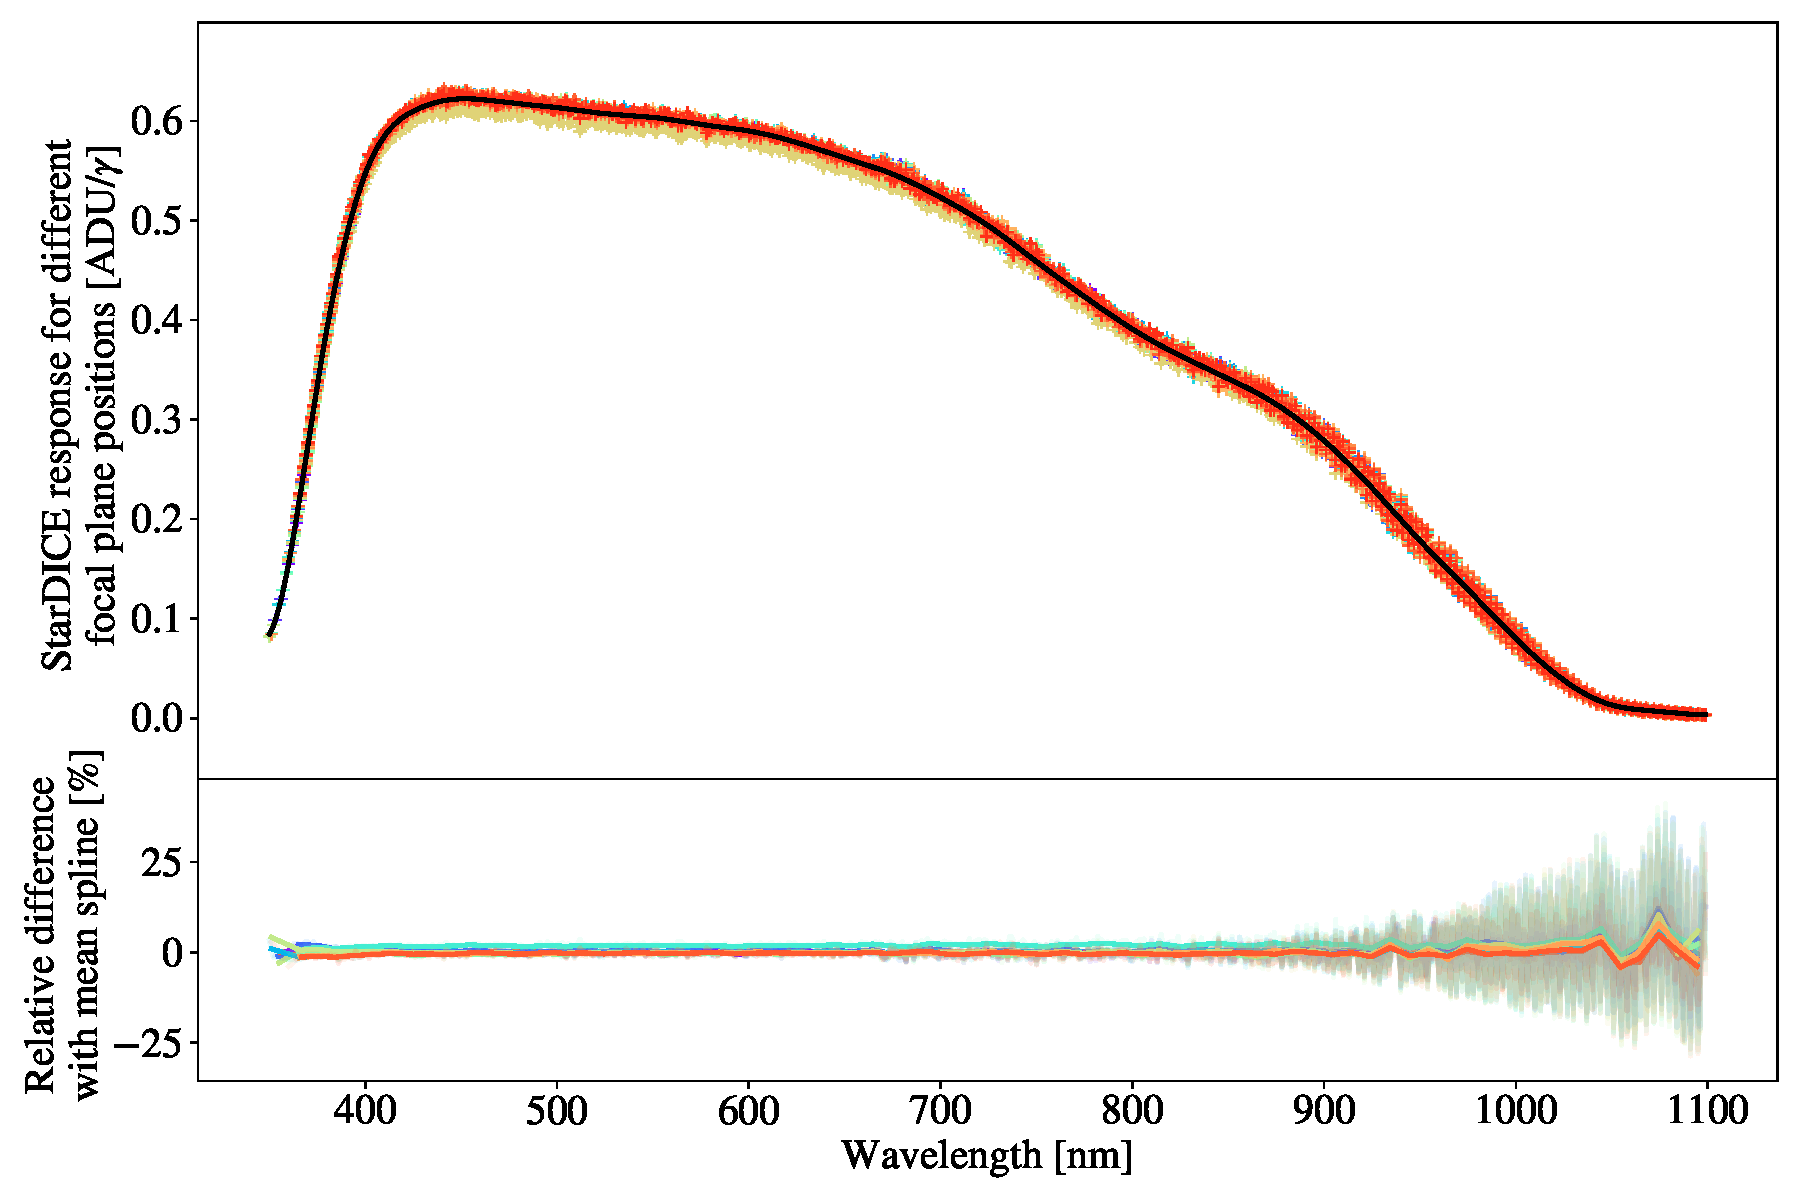
\includegraphics[width=\columnwidth]{fig/ccd_positions.pdf}
    \caption{Top : \SD response for the different positions on the focal plane, but same position on the mirror. Bottom : Relative difference between the data and the mean spline.}
    \label{fig:ccd_positions}
    %~/stardice/analysis/cbp_paper/golden_sample_analysis/dr2/2022_03_09_stardice_transmission_grid_auto.ipynb
\end{figure}

\subsection{Systematic uncertainties}
\label{sec:systematics}

\subsubsection{Stability of the StarDice responses}

\subsubsection{Gain and linearity}
\label{sec:gain}

Varying pinhole with StarDice, and CBP
Varying QSW but depending on result it falls into this subsection or the following

\subsubsection{Pinhole chromaticity}

\subsubsection{Pull distributions}

\subsubsection{Courbes de croissances}




